\documentclass[12pt]{amsart}
\usepackage{amsmath,amssymb,amsthm,amscd,appendix}
\usepackage[matrix,arrow,curve]{xy}

\usepackage{graphicx}
\usepackage{comment}
\usepackage{listings}
\usepackage{tikz}
\usepackage{changepage}
\usepackage[colorlinks=true,linkcolor=blue]{hyperref}
\usepackage[noabbrev]{cleveref}
\usepackage{overpic}
\usepackage{contour}

\hoffset=-26mm \frenchspacing \emergencystretch=5pt \tolerance=400
\unitlength=1mm \textwidth=17cm
%\renewcommand{\baselinestretch}{2}

\newtheorem{formula}{}[section]
\newtheorem{proposition}[formula]{Proposition}
\newtheorem{corollary}[formula]{Corollary}
\newtheorem{lemma}[formula]{Lemma}
\crefname{lemma}{Lemma}{Lemmas}
\newtheorem{theorem}[formula]{Theorem}
\newtheorem{conjecture}[formula]{Conjecture}
\newtheorem*{theorem*}{Theorem}


\theoremstyle{definition}
\newtheorem{definition}[formula]{Definition}
\crefname{definition}{Def.}{Definitions}
\newtheorem{construction}[formula]{Construction}
\newtheorem{example}[formula]{Example}
\newtheorem{notation}[formula]{Notation}

\theoremstyle{remark}
\newtheorem{remark}[formula]{Remark}
\crefname{remark}{Remark}{Remarks}
\newtheorem{problem}[formula]{Problem}
\newtheorem{question}[formula]{Question}
\newtheorem*{problem*}{Problem}

\crefname{section}{Section}{sections}
\crefname{figure}{Figure}{figures}
\crefname{equation}{}{equations}
\crefname{appendix}{Appendix}{}


\DeclareMathOperator{\cc}{cc}
\newcommand{\zp}{\mathcal Z_P}
\newcommand{\rp}{\mathcal R_P}
\newcommand{\zk}{\mathcal Z_K}

\newcommand{\mb}[1]{{\textbf {\textit#1}}}% bold italic letters

\begin{document}
 %\baselineskip=11pt
% \setcounter{page}{463}


\title[Generalization of OI-Type Kokotsakis Flexible Polyhedra]{Generalization of the Orthodiagonal Involutive Type of Kokotsakis Flexible Polyhedra}
\author{Alisher Aikyn, Yang Liu, Dmitry A.~Lyakhov, Helmut Pottmann, Dominik L.~Michels}

\address{Lomonosov Moscow State University, Kazakhstan Branch, Kazakhstan}
\email{aikyn.alisher@gmail.com}

\address{KAUST, Visual Computing Center, Kingdom of Saudi Arabia}
\email{dmitry.lyakhov@kaust.edu.sa}
\email{helmut.pottmann@kaust.edu.sa}
\email{dominik.michels@kaust.edu.sa}

\def\sgn{\mathrm{sgn}\,}
\def\bideg{\mathrm{bideg}\,}
\def\tdeg{\mathrm{tdeg}\,}
\def\sdeg{\mathrm{sdeg}\,}
\def\grad{\mathrm{grad}\,}
\def\ch{\mathrm{ch}\,}
\def\sh{\mathrm{sh}\,}
\def\th{\mathrm{th}\,}
\def\RZ{\mathbb{R}\mathcal{Z}}
\def\mod{\mathrm{mod}\,}
\def\In{\mathrm{In}\,}
\def\Im{\mathrm{Im}\,}
\def\Ker{\mathrm{Ker}\,}
\def\Hom{\mathrm{Hom}\,}
\def\Tor{\mathrm{Tor}\,}
\def\rk{\mathrm{rk}\,}
\def\codim{\mathrm{codim}\,}

\def\ko{{\mathbf k}}
\def\sk{\mathrm{sk}\,}
\def\RC{\mathrm{RC}\,}
\def\gr{\mathrm{gr}\,}

\def\R{{\mathbb R}}
\def\C{{\mathbb C}}
\def\Z{{\mathbb Z}}
\def\A{{\mathcal A}}
\def\B{{\mathcal B}}
\def\K{{\mathcal K}}
\def\M{{\mathcal M}}
\def\N{{\mathcal N}}
\def\E{{\mathcal E}}
\def\G{{\mathcal G}}
\def\D{{\mathcal D}}
\def\F{{\mathcal F}}
\def\L{{\mathcal L}}
\def\V{{\mathcal V}}
\def\H{{\mathcal H}}

%\newcommand{\rk}{\mathcal R_K}

%\subjclass[2010]{
%???
%}

\keywords{Kokotsakis polyhedron, skew-quad faces, spherical linkages, flexible quad mesh, orthodiagonal involutive type}

\begin{abstract}
In this paper we introduce and study a remarkable class of mechanisms formed by a $3 \times 3$ arrangement of rigid
and skew quadrilateral faces with revolute joints at the common edges. These Kokotsakis-type mechanisms with a quadrangular base and non-planar faces are a generalization of Izmestiev's orthodiagonal involutive type of
Kokotsakis polyhedra formed by planar quadrilateral faces. Our algebraic approach yields a complete characterization of all complexes of the orthodiagonal involutive type. It is shown that one has 8 degrees of freedom
to construct such mechanisms. This is illustrated by several examples, including cases that are not possible with planar
faces.

%In contrast to the planar case, 
%\textcolor{red}{two involutive couplings which contain deltoid and antideltoid respectively could be connected to mechanism demonstrating the rich geometry of the obtained case.}

%deltoids and antideltoids may be coupled \textcolor{orange}{involutively} demonstrating the rich geometry of the obtained mechanism.
\end{abstract}
\maketitle

\setcounter{section}{0}
%%%%%%%%%%%%%%%%%%%%%%%%%%%%%%%%%%%%%%%%%%%%%%%%%
\section{Introduction}
%%%%%%%%%%%%%%%%%%%%%%%%%%%%%%%%%%%%%%%%%%%%%%%%%

The growing interest in flexible or deployable structures is rooted in their wide-spread utility from robotics to solar cells, meta-materials, architecture and art. In the latter case, one also speaks of transformable design. One aims at a continuous morphing between different states of a shape, where the properties of these shapes and the motion depend on the targeted application.
Deployable structures may have a flat state or collapse even to a straight or curve-like shape. Even when confining
to rigid components of the structure, there is a wide variety of recent research: We mention
rigid-foldable origami \cite{demaine-book,evans2015,evans2016,ciang-2019-cf,song-2017,Tac09a,Tac10a,tachi-2010,tachi-2011-onedof,tachi-2013-composite,tachi2016} and its use to approximate given target surfaces 
\cite{dang-feng,feng-dang,dang2022inverse}, or so-called programmable meta-materials which are based on special
patterns and essentially constitute mechanisms, typically with many degrees of freedom \cite{Callens2018,dieleman2020,Dudte2016,auxetic-2022,Konakovic:2016:BDC:2897824.2925944,konakovic2018,silverberg2014}.

The present work is a step towards transformable design with quad mesh mechanisms. These are quad meshes
with regular combinatorics, possibly apart from a few isolated combinatorial singularities. Their faces
are rigid and the edges are revolute joints. If one goes beyond so-called elementary cells formed by a $3 \times 3$ grid
of quads, only very few solutions are known, especially if they do not possess a flat state as in origami.
These quad meshes have planar faces and are discrete counterparts of well-studied smooth surfaces, namely
Voss surfaces (characterized by a conjugate net of geodesics) \cite{voss1888uber} and profile affine surfaces
\cite{sauer-graf,sauer:1970} which generalize molding surfaces that are traced out by a planar profile whose plane
rolls on a cylinder. The discrete counterparts of Voss surfaces, so-called Voss nets are reciprocal parallel to
discrete models for surfaces of constant negative Gauss curvature  \cite{wunderlich-1951,sauer:1970}. Discrete profile
affine surfaces are known as T-nets, as their flat faces are all trapezoids. Both types have recently received
interest for applications in transformable design and architecture \cite{voss-IASS,t-nets-IASS,Mitchell2018,archdaily18}.


Flexible polyhedra have a long history in mathematical research. Famous examples include Bricard's flexible octahedra
\cite{bricard1897} and the flexible Kokotsakis polyhedra \cite{kokotsakis33,stachel2010}. The latter have a planar n-gon $P$ in the center, which is
surrounded by a belt of planar faces so that 3 faces meet at each vertex of $P$.  The case with a central quad $P$ 
is equivalent to a flexible $(3 \times 3)$ mesh of planar quads. A classification of all types of such meshes has been
given by Izmestiev \cite{izmestiev-2017}. According to Schief et al. \cite{Schief2008}, a quad mesh is flexible if and only
if all $3 \times 3$ submeshes are. However, the extension of Izmestiev's types to such larger flexible quad mesh
mechanisms is an unexplored area. To our best knowledge, the only known cases are still the classical Voss and T-nets. 

Another stream of relevant research is related to infinitesimal flexibility. Sauer \cite{sauer:1970} studied first
order flexibility in great detail, not only for the case of planar quad faces. However, he 
mentions that there is no known example for finite flexibility in the presence of non-planar faces. 
Schief et al. \cite{Schief2008} showed that in the smooth limit and for planar faces, second order infinitesimal flexibility
implies finite flexibility. This is not true for the discrete setting, but one has a remarkable
type of integrable systems \cite{Schief2008}. 

The first example of a flexible mesh with non-planar faces has recently been presented by Nawratil \cite{nawratil-2022,Nawratil2022}
in a study of generalized Kokotsakis belts with skew quads surrounding the central polyline. This is a generalization of the isogonal type in the planar quad case, where in each vertex both pairs of opposite angles are equal (as in Voss nets) or
supplementary (as in flat foldable origami). 

In the present paper, we present a larger novel class of flexible $(3 \times 3)$ complexes with skew quad faces. 
We refer to these generalized Kokotsakis meshes
with quadrangular bases and non-planar faces as skew-quad (SQ) Kokotsakis meshes. 
We follow the classical approach proposed by Bricard in order to reformulate the flexibility problem in Euclidean space to  one on sphere. This means that we can proceed with the polynomial system expressed in new variables, half-tangents of adjacent dihedral angles. Flexibility then means the existence of a one-parameter real-valued solution set of this
system.

We extend the approach of Izmestiev by constructing one remarkable class, more precisely of orthodiagonal spherical quadrilaterals with involutive couplings. We derive explicit algebraic expressions for constructing flexible $(3 \times 3)$ complexes. Moreover, these mechanisms have 8 degree of freedoms (which is wider in comparison to the planar case) and possess special geometric properties which generalize classical ones of T-hedra.

%%%%%%%%%%%%%%%%%%%%%%%%%%%%%%%%%%%%%%%%%%%%%%%%%%%%%%%%%%%%%%%%%%%%%%%%%%
\section{Configuration space of a spherical four-bar linkage}\label{sec2}
%%%%%%%%%%%%%%%%%%%%%%%%%%%%%%%%%%%%%%%%%%%%%%%%%%%%%%%%%%%%%%%%%%%%%%%%%%%%

The main object under consideration in this paper is a \emph{Kokotsakis polyhedron with a quad base and skew faces}. When referring to a Kokotsakis polyhedron we always mean this kind of object. We will present new flexible structures of this type. 

\subsection{Notations}
\begin{figure}[ht]
    \centering
    \begin{minipage}{0.5\textwidth}
        \centering
         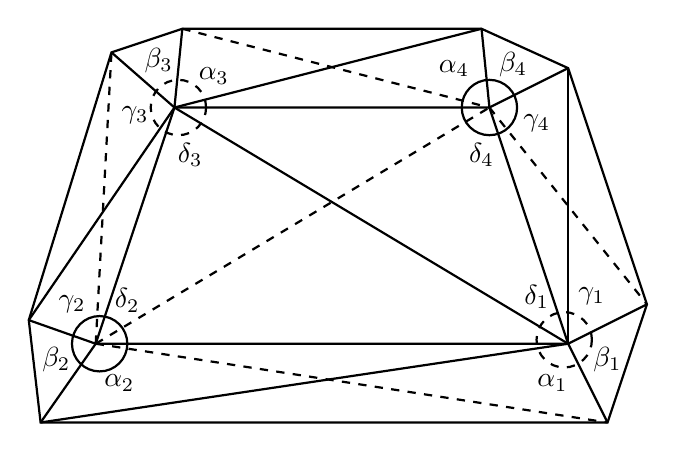
\begin{tikzpicture}[>=latex]                %\draw[help lines] (0,0) grid (15,10);

        \coordinate (a1) at (9, 4);
        \coordinate (a2) at (3, 4);
        \coordinate (a3) at (4, 7);
        \coordinate (a4) at (8, 7);
        \coordinate (b1) at (10, 4.5);
        \coordinate (c1) at (9.5, 3);
        \coordinate (b2) at (2.3, 3);
        \coordinate (c2) at (2.15, 4.3);
        \coordinate (b3) at (3.2, 7.7);
        \coordinate (c3) at (4.1, 8);
        \coordinate (b4) at (7.9, 8);
        \coordinate (c4) at (9, 7.5);

        \draw[thick] (a1) -- (a2) -- (a3) -- (a4) -- cycle;
        
        \draw[dashed, thick] (a2) -- (a4);
        \draw[thick] (a3) -- (a1);
        
        
        \draw[thick] (b1) -- (c1) -- (b2) -- (c2) -- (b3) -- (c3) -- (b4) -- (c4) -- cycle;
        
        \draw[thick] (a1) -- (b1);
        \draw[thick] (a1) -- (c1);
        
        \draw[thick] (a2) -- (b2);
        \draw[thick] (a2) -- (c2);
        
        \draw[thick] (a3) -- (b3);
        \draw[thick] (a3) -- (c3);

        \draw[thick] (a4) -- (b4);
        \draw[thick] (a4) -- (c4);

        \draw[thick] (a1) -- (c4); 
        \draw[thick, dashed] (a4) -- (b1);
        
        \draw[thick, dashed] (a2) -- (c1);
        \draw[thick] (a1) -- (b2);

        \draw[thick, dashed] (a2) -- (b3);
        \draw[thick] (c2) -- (a3);

        \draw[thick, dashed] (c3) -- (a4);
        \draw[thick] (b4) -- (a3);

        \draw[thick, dashed] (a1) + (-0.05,0.05) circle (10pt);
        \draw (8.6, 4.6) node {$\delta_1$};
        \draw (9.3, 4.6) node {$\gamma_1$};
        \draw (9.5, 3.8) node {$\beta_1$};
        \draw (8.8, 3.5) node {$\alpha_1$};

        \draw[thick] (a2) + (0.05,0) circle (10pt);
        \draw (a2) + (0.4, 0.55) node {$\delta_2$};
        \draw (a2) + (-0.3, 0.5) node {$\gamma_2$};
        \draw (a2) + (-0.5, -0.2) node {$\beta_2$};
        \draw (a2) + (0.3, -0.5) node {$\alpha_2$};

        \draw[thick, dashed] (a3) + (0.05,0) circle (10pt);
        \draw (a3) + (0.2, -0.6) node {$\delta_3$};
        \draw (a3) + (0.5, 0.4) node {$\alpha_3$};
        \draw (a3) + (-0.2, 0.6) node {$\beta_3$};
        \draw (a3) + (-0.5, -0.1) node {$\gamma_3$};
        
        \draw[thick] (a4) circle (10pt);
        \draw (a4) + (-0.1, -0.6) node {$\delta_4$};
        \draw (a4) + (0.3, 0.55) node {$\beta_4$};
        \draw (a4) + (-0.45, 0.5) node {$\alpha_4$};
        \draw (a4) + (0.
        6, -0.2) node {$\gamma_4$};
        
    \end{tikzpicture}
    \end{minipage}\hfill
    \begin{minipage}{0.5\textwidth}
        \centering
        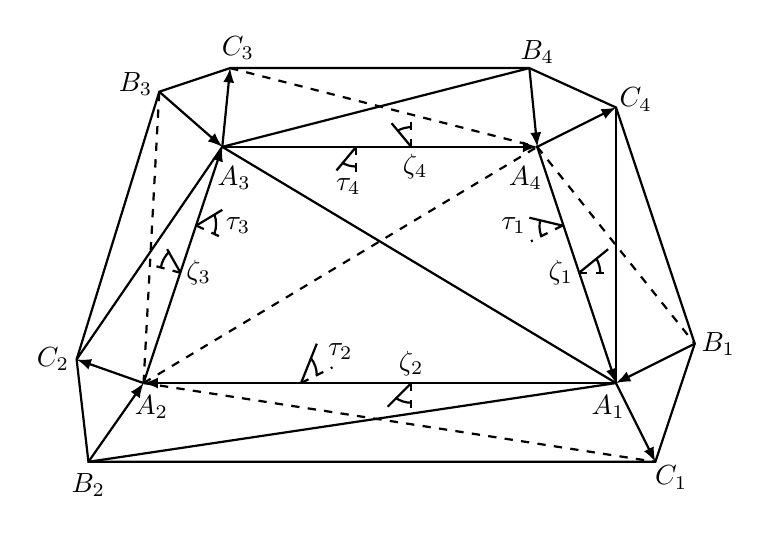
\begin{tikzpicture}[>=latex]              %\draw[help lines] (0,0) grid (15,10);

        \coordinate (a1) at (9, 4);
        \coordinate (a2) at (3, 4);
        \coordinate (a3) at (4, 7);
        \coordinate (a4) at (8, 7);
        \coordinate (b1) at (10, 4.5);
        \coordinate (c1) at (9.5, 3);
        \coordinate (b2) at (2.3, 3);
        \coordinate (c2) at (2.15, 4.3);
        \coordinate (b3) at (3.2, 7.7);
        \coordinate (c3) at (4.1, 8);
        \coordinate (b4) at (7.9, 8);
        \coordinate (c4) at (9, 7.5);

        \draw[thick] (a1) edge[->] (a2) (a2) edge[->] (a3) (a3) edge[->] (a4) (a4) edge[->] (a1);
        
        \draw[dashed, thick] (a2) -- (a4);
        \draw[thick] (a3) -- (a1);
        
        
        \draw[thick] (b1) -- (c1) -- (b2) -- (c2) -- (b3) -- (c3) -- (b4) -- (c4) -- cycle;
        
        \draw[thick, <-] (a1) -- (b1);
        \draw[thick, ->] (a1) -- (c1);
        
        \draw[thick, <-] (a2) -- (b2);
        \draw[thick, ->] (a2) -- (c2);
        
        \draw[thick, <-] (a3) -- (b3);
        \draw[thick, ->] (a3) -- (c3);

        \draw[thick, <-] (a4) -- (b4);
        \draw[thick, ->] (a4) -- (c4);

        \draw[thick] (a1) -- (c4); 
        \draw[thick, dashed] (a4) -- (b1);
        
        \draw[thick, dashed] (a2) -- (c1);
        \draw[thick] (a1) -- (b2);

        \draw[thick, dashed] (a2) -- (b3);
        \draw[thick] (c2) -- (a3);

        \draw[thick, dashed] (c3) -- (a4);
        \draw[thick] (b4) -- (a3);

        \draw (a1) + (-0.1, -0.3) node {$A_1$};
        \draw (b1) + (0.3, 0) node {$B_1$};
        \draw (c1) + (0.2, -0.2) node {$C_1$};
        
        \draw (a2) + (0.1, -0.3) node {$A_2$};
        \draw (b2) + (0, -0.3) node {$B_2$};
        \draw (c2) + (-0.3, 0) node {$C_2$};
        
        \draw (a3) + (0.15, -0.4) node {$A_3$};
        \draw (b3) + (-.3, 0.1) node {$B_3$};
        \draw (c3) + (0.1, .25) node {$C_3$};
        
        \draw (a4) + (-0.15, -0.4) node {$A_4$};
        \draw (b4) + (0.1, 0.2) node {$B_4$};
        \draw (c4) + (.25, .1) node {$C_4$};

        \draw[thick, dashed] (5, 4) -- (5.4, 4.2);
        \draw[thick] (5, 4) -- (5.2, 4.5);
        \draw[thick] (5.2,4.1) arc (0:39:10pt);
        \draw (5.5, 4.4) node {$\tau_2$};

        \draw[thick] (6.4, 4) -- (6.1, 3.7);
        \draw[thick, dashed] (6.4, 4) -- (6.4, 3.65);
        \draw[thick] (6.4, 3.75) arc (270:235:10pt);
        \draw (6.4, 4.25) node {$\zeta_2$};

        \draw[thick] (8.53, 5.4) -- (8.9, 5.7);
        \draw[thick, dashed] (8.53, 5.4) -- (8.9, 5.4);
        \draw[thick] (8.8, 5.4) arc(0:30:10pt);
        \draw (8.3, 5.4) node {$\zeta_1$};

        \draw[thick, dashed] (8.32, 6) -- (7.92, 5.8);
        \draw[thick] (8.32, 6) -- (7.9, 6.1);
        \draw[thick] (8.05, 5.87) arc(200:167:10pt);
        \draw[thick] (7.7, 6) node {$\tau_1$};
        
        \draw[thick] (6.4, 7) -- (6.15, 7.3);
        \draw[thick, dashed] (6.4, 7) -- (6.4, 7.4);
        \draw[thick] (6.4, 7.25) arc (90:120:10pt);
        \draw (6.45, 6.75) node {$\zeta_4$}; 

        \draw[thick, dashed] (5.7, 7) -- (5.7, 6.6);
        \draw[thick] (5.7, 7) -- (5.45,6.7);
        \draw[thick] (5.7, 6.75) arc(270:240: 10pt);
        \draw (5.6, 6.5) node {$\tau_4$};

        %\draw[thick] (3.7, 6) node {\textbullet};
        \draw[thick, dashed] (3.47, 5.4) -- (3.1, 5.5);
        \draw[thick] (3.47, 5.4) -- (3.3, 5.7);
        \draw[thick] (3.22, 5.47) arc(170:132:10pt);
        \draw (3.7, 5.4) node {$\zeta_3$};

        \draw[thick] (3.67, 6) -- (4, 6.2);
        \draw[thick, dashed, rotate around ={-25:(3.67, 6)} ] (3.67, 6) -- (4, 6);
        \draw[thick] (3.9, 5.9) arc (-20:20:10pt);
        \draw (4.2, 6) node {$\tau_3$};
    \end{tikzpicture} % second figure itself
    \end{minipage}
    \caption{Angles and vertices in a skew Kokotsakis polyhedron with a quad base}\label{fig1}
\end{figure}
In this subsection we describe the notations of angles in order to transform the geometrical problem into algebra. We interpret every skew quad as a rigid tetrahedron. The enumeration of vertices and angles is cyclic and takes values from $\{1\ldots 4\}$.  

We denote by $\alpha_i, \beta_i, \gamma_i, \delta_i \in (0, \pi)$ the angles between edges as shown in \cref{fig1}. Each $\delta_i$ is the angle between edges $A_{i - 1}A_{i}, A_{i}A_{i - 1}$, $\beta_i$ is the angle between $B_{i}A_i, A_{i}C_{i}$, $\alpha_i$ is the angle between $C_{i}A_{i}, A_i A_{i+1}$ if $i = 1, 3$ and $B_i A_i, A_i A_{i - 1}$ if $i = 2, 4$, $\gamma_i$ is the angle between $B_i A_i, A_i A_{i - 1}$ if $i = 1, 3$ and $C_i A_i, A_i A_{i + 1}$ if $i = 2, 4$. They play the same role as the  planar angles in \cite{izmestiev-2017}.

In the analysis of flexibility of the non-planar case, we have to consider the dihedral angles of all tetrahedrons as well. Denote by $a_i = A_{i - 1} A_i$, $b_i = B_i A_i$, $c_i = A_i C_i$, where for two points $A$ and $B$, $AB$ is the vector from point $A$ to point $B$. We fix the orientation such that $a_1, a_2, [a_1, a_2]$ are positively oriented, where $[a, b]$ is the cross product of vectors $a, b$. By $\tau_i, \zeta_i \in (-\pi, \pi)$ we denote the fixed oriented dihedral angles of the central tetrahedron $A_1 A_2 A_3 A_4$ and side tetrahedrons, respectively, as in \cref{fig1}. Each $\tau_i$ is the angle between faces $[A_{i - 2}, A_{i-1}, A_{i}], [A_{i - 1} A_i A_{i+1}]$, $\zeta_i$ is the angle between faces $[C_{i - 1}, A_{i - 1}, A_{i}], [A_{i - 1}, A_{i}, B_i]$. By $\phi_i, \psi_i \in (-\pi, \pi)$ we denote the flexible oriented dihedral angles as in \cref{fig2}.

We can calculate these angles with signs as follows:
\begin{equation*}
    \tau_i = \text{sign}(o)\arccos\frac{([a_{i - 1}, a_i], [a_i, a_{i + 1}])}{\lVert[a_{i - 1}, a_i]\rVert \lVert[a_{i}, a_{i + 1}]\rVert}, \quad \text{where} \quad o = \begin{cases}
    \cos([a_i, a_{i + 1}], a_{i + 2}), \text{ if } i = 1, 3\\
    \cos([a_{i - 1}, a_{i}],a_{i + 1}), \text{ if } i = 2, 4
    \end{cases}
\end{equation*}
\begin{equation*}
    \zeta_i = \text{sign}(o)\arccos\frac{([a_{i}, b_i], [c_{i - 1}, a_{i}])}{\Vert[a_{i},b_i]\Vert \Vert[c_{i - 1}, a_i]\Vert} \quad \text{where} \quad o = 
    \begin{cases}
        \cos([a_i, b_i], c_i), \text{ if } i = 1, 3\\
        \cos([c_{i - 1}, a_i], b_i), \text{ if } i = 2, 4\\
    \end{cases}
\end{equation*}
\begin{equation*}
    \phi_i = 
    \begin{cases}
        \text{sign}(\cos([a_i, a_{i + 1}], b_i))\arccos\frac{([a_i, a_{i + 1}], [a_{i}, b_{i}])}{\Vert[a_i, a_{i + 1}]\Vert \Vert[a_{i}, b_{i}]\Vert}, \text{ if } i = 1, 3\\
        \text{sign}(\cos([a_{i - 1}, a_{i}], c_{i - 1}))\arccos\frac{([a_{i - 1}, a_{i}], [c_{i- 1}, a_{i}])}{\Vert[a_{i - 1}, a_{i}]\Vert \Vert[c_{i - 1}, a_{i}]\Vert}, \text{ if } i = 2, 4
    \end{cases}
\end{equation*}
\begin{equation*}
    \psi_i =
    \begin{cases}
        \text{sign}(\cos([a_{i - 1}, a_i], c_{i - 1}))\arccos{\frac{([a_{i - 1}, a_i], [c_{i - 1}, a_i])}{\Vert[a_{i - 1}, a_i]\Vert \Vert[c_{i - 1}, a_i]\Vert}}, \text{ if } i = 1, 3\\
        \text{sign}(\cos([a_{i}, a_{i + 1}], b_i)) \arccos{\frac{([a_i, a_{i + 1}], [a_i, b_i])}{\Vert[a_{i}, a_{i + 1}]\Vert \Vert[a_i, b_i]\Vert}}, \text{ if } i = 2, 4,
    \end{cases}
\end{equation*}
where $(\cdot, \cdot)$ defines the dot product of vectors.

Changing the dihedral angles $\phi_i$ and $\psi_i$, shown in \cref{fig2}, corresponds to the flexibility property of the Kokotsakis polyhedron. Angles $\phi_i$ and $\psi_i$ are the dihedral angles between the corresponding planes of the central and the side tetrahedrons. The dihedral angles satisfy the equality $\psi_i = \phi_i + \tau_i + \zeta_i$. Indeed, since $\psi_1$ is the angle between planes $[C_4 A_4 A_1], [A_3 A_4 A_1]$ and $\tau_1$ is the angle between planes $[A_3 A_4 A_1], [A_4 A_1 A_2]$, then $\psi_1 - \tau_1$ is equal to $\phi_1 + \zeta_1$, where $\phi_1$ is the angle between planes $[A_4 A_1 A_2], [A_4 A_1 B_1]$ and $\zeta_1$ is the angle between planes $[C_4 A_4 A_1], [A_4 A_1 B_1]$. The same holds for other indices.
\begin{figure}[ht]
    \centering
    \begin{minipage}{0.5\textwidth}
        \centering
            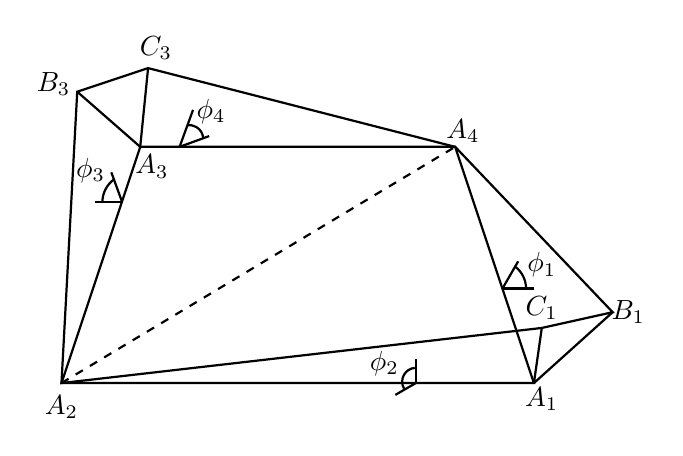
\begin{tikzpicture}[>=latex]           %   \draw[help lines] (0,0) grid (15,10);

        \coordinate (a1) at (9, 4);
        \coordinate (a2) at (3, 4);
        \coordinate (a3) at (4, 7);
        \coordinate (a4) at (8, 7);
        \coordinate (b1) at (10, 4.9);
        \coordinate (c1) at (9.1, 4.7);
        \coordinate (b2) at (2.3, 3);
        \coordinate (c2) at (2.15, 4.3);
        \coordinate (b3) at (3.2, 7.7);
        \coordinate (c3) at (4.1, 8);
        \coordinate (b4) at (7.9, 8);
        \coordinate (c4) at (9, 7.5);

        \draw[thick] (a1) -- (a2) -- (a3) -- (a4) -- cycle;
        
        \draw[dashed, thick] (a2) -- (a4);
        
        
        \draw[thick] (b1) -- (c1) -- (a2) -- (b3) -- (c3) -- (a4) -- cycle;
        
        \draw[thick] (a1) -- (b1);
        \draw[thick] (a1) -- (c1);
    
        \draw[thick] (a3) -- (b3);
        \draw[thick] (a3) -- (c3);

        \draw (a1) + (0.1, -0.2) node {$A_1$};
        \draw (b1) + (0.2, 0) node {$B_1$};
        \draw (c1) + (0, 0.25) node {$C_1$};
        
        \draw (a2) + (0, -0.3) node {$A_2$};
        
        \draw (a3) + (0.15, -0.25) node {$A_3$};
        \draw (b3) + (-.3, 0.1) node {$B_3$};
        \draw (c3) + (0.1, .25) node {$C_3$};
        
        \draw (a4) + (0.1, 0.2) node {$A_4$};
        
        \draw[thick] (7.5, 4) -- (7.5, 4.3);
        \draw[thick, rotate around = {30:(7.5, 4)}] (7.5, 4) -- (7.2, 4);
        \draw[thick] (7.35, 3.93) arc (210:95:5pt);
        \draw (7.1, 4.25) node {$\phi_2$};
        
        \draw[thick] (8.6, 5.2) -- (9, 5.2);
        \draw[thick, rotate around = {60:(8.6, 5.2)}] (8.6, 5.2) -- (9, 5.2);
        \draw[thick] (8.9, 5.2) arc (0:51:10pt);
        \draw (9.1, 5.5) node {$\phi_1$};

        \draw[thick, rotate around = {20:(4.5, 7)}] (4.5, 7) -- (4.9, 7);
        \draw[thick, rotate around = {70:(4.5, 7)}] (4.5, 7) -- (5, 7);
        \draw[thick] (4.8, 7.1) arc (0:100:5pt);
        \draw (4.9, 7.45) node {$\phi_4$};

        %\draw (3.75, 6.3) node {\textbullet};
        \coordinate (phi3) at (3.77, 6.3);
        \draw[thick, rotate around = {-70:(phi3)}] (phi3) -- + (-0.4,0);
        \draw[thick] (phi3) -- + (-0.35, 0);
        \draw[thick] (phi3) + (-0.25, 0) arc (180:125:10pt);
        \draw (phi3) + (-0.4,0.4) node {$\phi_3$};
        
     \end{tikzpicture}
    \end{minipage}\hfill
    \begin{minipage}{0.5\textwidth}
        \centering
        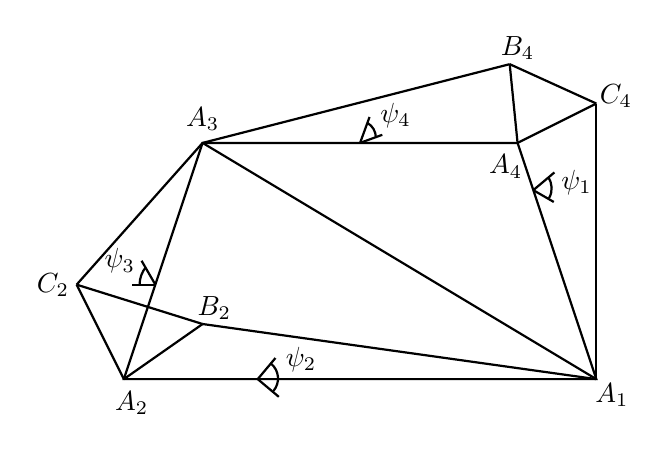
\begin{tikzpicture}[>=latex]              %\draw[help lines] (0,0) grid (15,10);

        \coordinate (a1) at (9, 4);
        \coordinate (a2) at (3, 4);
        \coordinate (a3) at (4, 7);
        \coordinate (a4) at (8, 7);
        \coordinate (b1) at (10, 4.5);
        \coordinate (c1) at (9.5, 3);
        \coordinate (b2) at (4, 4.7);
        \coordinate (c2) at (2.4, 5.2);
        \coordinate (b3) at (3.2, 7.7);
        \coordinate (c3) at (4.1, 8);
        \coordinate (b4) at (7.9, 8);
        \coordinate (c4) at (9, 7.5);

        \draw[thick] (a1) -- (a2) -- (a3) -- (a4) -- cycle;
        
        \draw[thick] (a3) -- (a1);
        \draw[thick] (a2) -- (b2);
        \draw[thick] (a2) -- (c2);
        \draw[thick] (a4) -- (b4);
        \draw[thick] (a4) -- (c4);
        \draw[thick] (a1) -- (c4); 
        \draw[thick] (a1) -- (b2);
        \draw[thick] (c2) -- (a3);
        \draw[thick] (b4) -- (a3);
        \draw[thick] (b2) -- (c2);
        \draw[thick] (b4) -- (c4);

        \draw (a1) + (0.2, -0.2) node {$A_1$};
        
        \draw (a2) + (0.1, -0.3) node {$A_2$};
        \draw (b2) + (0.15, 0.2) node {$B_2$};
        \draw (c2) + (-0.3, 0) node {$C_2$};
        
        \draw (a3) + (0, 0.3) node {$A_3$};
        
        \draw (a4) + (-0.15, -0.3) node {$A_4$};
        \draw (b4) + (0.1, 0.2) node {$B_4$};
        \draw (c4) + (.25, .1) node {$C_4$};

        \coordinate (psi2) at (4.7, 4);
        \draw[thick, , rotate around = {-40:(psi2)}] (psi2) -- + (0, 0.35);
        \draw[thick, rotate around = {-40:(psi2)}] (psi2) -- + (0.35, 0);
        \draw[thick] (psi2) + (0.2, -0.15) arc (-40:50:7pt);
        \draw (psi2) + (0.55, 0.25) node {$\psi_2$};

        \coordinate (psi3) at (3.4, 5.2);
        %\draw (psi3) node {\textbullet};
        \draw[thick, , rotate around = {30:(psi3)}] (psi3) -- + (0, 0.35);
        \draw[thick, , rotate around = {0:(psi3)}] (psi3) -- + (-0.3, 0);
        \draw[thick] (psi3) + (-0.2, 0) arc (180:141:10pt);
        \draw (psi3) + (-0.45, 0.3) node {$\psi_3$};

        \coordinate (psi1) at (8.2, 6.4);
        %\draw (psi4) node {\textbullet};
        \draw[thick, rotate around = {-50:(psi1)}] (psi1) -- + (0, 0.35);
        \draw[thick, rotate around = {-30:(psi1)}] (psi1) -- + (0.3, 0);
        \draw[thick] (psi1) + (0.2, -0.1) arc (-30:36:7pt);
        \draw (psi1) + (.55, .1) node {$\psi_1$};

        \coordinate (psi4) at (6, 7);
        %\draw (psi4) node {\textbullet};
        \draw[thick, rotate around = {-20:(psi4)}] (psi4) -- + (0, 0.35);
        \draw[thick, rotate around = {20:(psi4)}] (psi4) -- + (0.3, 0);
        \draw[thick] (psi4) + (0.2, .07) arc (0:60:6pt);
        \draw (psi4) + (.45, .35) node {$\psi_4$};
        
    \end{tikzpicture} % second figure itself
    \end{minipage}
    \caption{Dihedral angles which change in a flexible Kokotsakis polyhedron}\label{fig2}
\end{figure}
\subsection{Spherical image}
In order to study the configuration space of Kokotsakis polyhedrons, we follow the classical approach of associating it with a movable spherical linkage (cf. \cite{izmestiev-2017}, \cite{nawratil-2010}, \cite{nawratil-2011}, \cite{nawratil-2012}, \cite{nawratil-2022} and \cite{stachel2010}). 
For each of the four interior vertices $A_1, A_2, A_3, A_4$ consider its spherical image, that is, the intersection of the cone of adjacent faces with a unit sphere centered at the vertex. This yields four spherical quadrilaterals $Q_i$ with side lengths $\alpha_i, \beta_i, \gamma_i, \delta_i$ in this cyclic order.  In the works mentioned above, the faces of a Kokotsakis polyhedron are planar and 
therefore the spherical images of two adjacent vertices are {\it coupled} by means of a common dihedral angle. However, since we have
skew quad faces, we have to consider a generalization of that definition, as introduced by Nawratil  \cite{nawratil-2022}. Spherical images of two adjacent vertices are {\it coupled} if the difference of their dihedral angles in the common vertices is constant during all deformations. Thus, for every edge $A_i A_{i+1}$ we have a scissors-like coupling of two spherical quadrilaterals, see \cref{fig5}.

A Kokotsakis polyhedron is flexible if and only if the spherical linkage that is formed by the closed chain of four coupled spherical images corresponding to the four edges of the base quad is flexible. Thus, in order to study flexible Kokotsakis polyhedrons, it suffices to consider all such flexible spherical linkages.


We start by recalling classical results about the configuration space of a spherical quadrilateral for the first quadrangle $Q_1$ in \cref{fig4}.
\begin{figure}[ht!]
    \centering
    \begin{minipage}{0.5\textwidth}
        \centering
            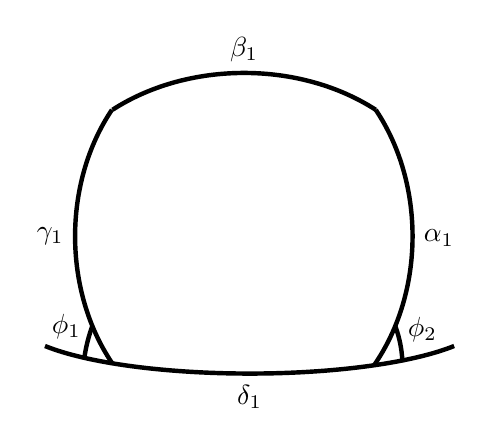
\begin{tikzpicture}
        \draw[ultra thick] (2.5, 2) arc[start angle=210, end angle = 330, x radius = 3cm, y radius = 0.7cm]  node[below, midway] {$\delta_1$};
        \draw[ultra thick] (3.35, 5) arc [start angle=140, end angle=220,x radius = 2cm, y radius = 2.5cm] node[left, midway] {$\gamma_1$};
        \draw[ultra thick] (6.7, 5) arc [start angle=40, end angle=-41,x radius = 2cm, y radius = 2.5cm] node[right, midway] {$\alpha_1$};
        \draw[ultra thick] (6.7,5) arc [start angle=50, end angle=130,x radius =2.6cm, y radius = 2cm] node[above, midway] {$\beta_1$};
        \draw[ultra thick] (3.1, 2.25) arc[start angle = 160, end angle = 172,radius=2cm] node[left, pos = 0] {$\phi_1$};
        \draw[ultra thick] (6.95, 2.25) arc[start angle = 20, end angle = 3,radius=1.5cm] node[right, pos = 0.1] {$\phi_2$};
       
    \end{tikzpicture}

        \caption{Spherical quadrangle $Q_1$}
        \label{fig4}
    \end{minipage}\hfill
    \begin{minipage}{0.5\textwidth}
        \centering
        \scalebox{0.8}{
    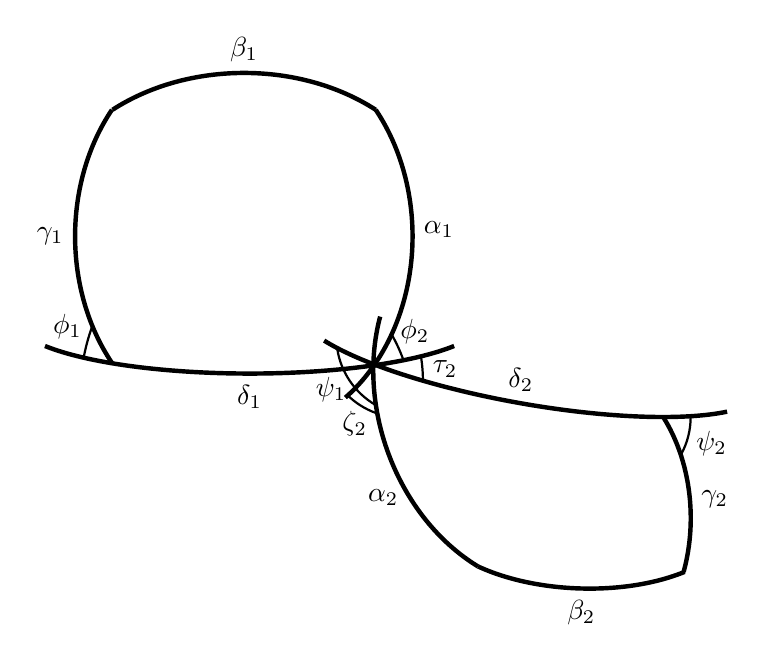
\begin{tikzpicture}
     \draw[ultra thick] (0.5, 2) arc[start angle=210, end angle = 330, x radius = 3cm, y radius = 0.7cm]  node[below, midway] {$\delta_1$};
        \draw[ultra thick] (1.35, 5) arc [start angle=140, end angle=220,x radius = 2cm, y radius = 2.5cm] node[left, midway] {$\gamma_1$};
        \draw[ultra thick] (4.7, 5) arc [start angle=40, end angle=-55,x radius = 2cm, y radius = 2.5cm] node[right, pos = 0.4] {$\alpha_1$};
        \draw[ultra thick] (4.7,5) arc [start angle=50, end angle=130,x radius =2.6cm, y radius = 2cm] node[above, midway] {$\beta_1$};
        \draw[thick] (1.1, 2.25) arc[start angle = 160, end angle = 170,radius=2.5cm] node[left, pos = 0] {$\phi_1$};
        \draw[thick] (4.9, 2.15) arc[start angle = 30, end angle = 20,radius=2cm] node[right, pos = -0.1] {$\phi_2$};
        
%        \node [red] at (11.7, 1.75) {\textbullet};
%        \node [red] at (15.35, 1.1) {\textbullet};
%        \node [green] at (13,-0.8) {\textbullet};
 %       \node [green] at (11.8, 1) {\textbullet};
        
        
        \draw[ultra thick, rotate around={-10:(4.7,1.75)}] (4, 1.95) arc [start angle=210, end angle = 330, x radius = 3cm, y radius = 0.7cm] node[above, midway] {$\delta_2$};
        \draw[ultra thick, rotate around = {19:(6,-0.8)}] (6,-0.8) arc [start angle=-134, end angle=-220,x radius = 2cm, y radius = 2.5cm] node[left, pos = 0.35] {$\alpha_2$};
        \draw[ultra thick, rotate around = {0:(8.35,1.1)}] (8.35,1.1) arc [start angle=40, end angle=-20,x radius = 1.5cm, y radius = 2cm] node[right, pos = 0.55] {$\gamma_2$};
        \draw[ultra thick, rotate around = {-2:(6,-0.8)}] (6,-0.8) arc [start angle=230, end angle=312,x radius = 2cm, y radius = 1cm] node[below, midway] {$\beta_2$};
        \draw[thick] (5.3, 1.55) arc[start angle = 0, end angle = 9,radius=2cm] node[right, pos = 0.5] {$\tau_2$};
        \draw[thick] (4.7, 1.25) arc[start angle = -120, end angle = -171,radius=1cm] node[left, pos = 0.35] {$\psi_1$};
        \draw[thick] (8.7, 1.1) arc[start angle = 0, end angle = -28, radius=1cm] node[right, pos = 0.7] {$\psi_2$};
        \draw[thick] (4.7, 1.15) arc[start angle = -110, end angle = -135, radius=1cm] node[below, pos = 0.7] {$\zeta_2$};
    \end{tikzpicture}
}
        \caption{A coupling $(Q_1, Q_2)$ of two quadrilaterals}
        \label{fig5}
    \end{minipage}
\end{figure}
A spherical quadrilateral $Q_1$ with given side lengths $(\alpha_1, \beta_1, \gamma_1, \delta_1)$ is uniquely determined by the values of two adjacent angles; on the other hand, these angles satisfy a certain relation.
By performing the substitution
\begin{equation}\label{eq1}
    x_1 = \tan\frac{\phi_1}{2}, \quad x_2 = \tan\frac{\phi_2}{2}, 
\end{equation}
where $\phi_1$ and $\phi_2$ are as in \cref{fig4}, this leads to a polynomial equation for $x_1$ and $x_2$.
\begin{lemma}[\cite{bricard1897}]
The configuration space of quadrilateral $Q_1$ with side lengths $\alpha_1$, $\beta_1$, $\gamma_1$, $\delta_1$ in this cyclic order is the solution of the equation
\begin{equation}\label{eq2}
P_1(x_{2}, x_1) = c_{22} x_{2}^2 x_1^2 + c_{20} x_{2}^2 + c_{02} x_1^2 + 2c_{11} x_{2} x_1 + c_{00} = 0,
\end{equation}
where
$$
\begin{matrix}
c_{22} = \sin \frac{\alpha_1 + \beta_1 + \gamma_1 - \delta_1}{2} \sin \frac{\alpha_1 - \beta_1 + \gamma_1 - \delta_1}{2}, \\
c_{20} = \sin \frac{\alpha_1 - \beta_1 - \gamma_1 - \delta_1}{2} \sin \frac{\alpha_1 + \beta_1 - \gamma_1 - \delta_1}{2}, \\
c_{02} = \sin \frac{\alpha_1 + \beta_1 - \gamma_1 + \delta_1}{2} \sin \frac{\alpha_1 - \beta_1 - \gamma_1 + \delta_1}{2}, \\
c_{11} = -\sin\alpha_1 \sin \gamma_1, \\
c_{00} = \sin \frac{\alpha_1 - \beta_1 + \gamma_1 + \delta_1}{2} \sin \frac{\alpha_1 + \beta_1 + \gamma_1 + \delta_1}{2}.
\end{matrix}
$$
\end{lemma}
The proof can be found in \cite{stachel2010}. We view equation \cref{eq2} as an equation in two projective variables $x_1, x_2 \in \mathbb{C}P^1$, to incorporate the value $\infty$ for $\phi_i=\pi$. By $Z_1$ we denote the solution set of \cref{eq2} in $(\mathbb{C}P^1)^2$
$$
Z_1 = \{(x_2, x_1) \in \mathbb{C}P^1 \times \mathbb{C}P^1|P_1(x_2, x_1) = 0\}.
$$
The same result holds for the other quads $Q_i$, which means that the configuration space of a Kokotsakis polyhedron equals the set of solutions for the system
\begin{equation}\label{eq3}
P_1(x_2, x_1) = 0, \quad P_2(y_2, y_3) = 0, \quad P_3(x_4, x_3) = 0, \quad P_4(y_4, y_1) = 0,
\end{equation}
where $x_i = \tan \frac{\phi_i}{2}$,  $y_i = \tan \frac{\psi_i}{2}$.
\begin{lemma}
A skew Kokotsakis polyhedron with a quad base is flexible if and only if the system of polynomial equations \cref{eq3} has a family of one-parameter solutions over the reals.
\end{lemma}
The approach used by Izmestiev in \cite{izmestiev-2017} for the case of planar faces (where $y_i = x_i$) was to find conditions when algebraic sets $R_{12}(x_1, x_3) = \text{res}_{x_2}(P_1, P_2) = 0$ and $R_{34}(x_1, x_3) = \text{res}_{x_4}(P_3, P_4) = 0$ have a common irreducible component, where $\text{res}_{x_k}(P_i, P_j)$ stands for a resultant with respect to $x_k$. We will follow the same approach in \cref{sec3}.
\subsection{Orthodiagonal quadrilateral}
Let $Q$ be a spherical quadrilateral with side lengths $\alpha, \beta, \gamma, \delta$ in this cyclic order. The form of configuration space of $Q$ depends on the number and the type of solutions of the equation
\begin{equation}\label{eq4}
\alpha \pm \beta \pm \gamma \pm \delta = 0\quad(\text{mod }2\pi)
\end{equation}
\begin{definition}
A spherical quadrilateral is said to be
    \begin{itemize}
        \item of {\it elliptic} type, if equation \cref{eq4} has no solutions;
        \item of {\it conic} type, if equation \cref{eq4} has exactly one solution;
        \item a {\it deltoid}, if it has two pairs of equal adjacent sides, and an {\it antideltoid}, if it has two pairs of adjacent sides complementing each other to $\pi$;
        \item an {\it isogram}, if pairs of opposite sides have equal lengths, and an antiisogram, if lengths of opposite sides complement each other to $\pi$.
    \end{itemize}
\end{definition}
Izmestiev \cite{izmestiev-2017}  described parametrizations of the configuration space of each of these types. We are only interested in the elliptic and deltoid cases.


A spherical quadrilateral is said to be {\it orthodiagonal}, if its diagonals are orthogonal. The orthodiagonality is equivalent to the following identity
    \begin{lemma}[Lemma 6.3, \cite{EI20}]\label{lma5.3}
        The diagonals of a spherical quadrilateral with side lengths $\alpha, \beta, \gamma, \delta$ (in this cyclic order) are orthogonal if and only if its side lengths satisfy the relation
        \begin{equation}\label{eq33}
            \cos \alpha \cos \gamma = \cos \beta \cos \delta.
        \end{equation}
    \end{lemma}

The orthodiagonality property is quite remarkable as it also implies an existence property:
    \begin{lemma}[Lemma 6.4, \cite{EI20}]
        Let $\alpha, \beta, \gamma, \delta \in (0, \pi)$ satisfy $\cos\alpha \cos \gamma = \cos \beta \cos \delta$. Then there exists a spherical orthodiagonal quadrilateral with side lengths $\alpha, \beta, \gamma, \delta$.
    \end{lemma}


\begin{lemma}[Lemma 4.12, \cite{izmestiev-2017}]\label{lma2.5}
If $Q_1$ is an orthodiagonal quadrilateral then it is either an (anti)deltoid or of the elliptic type.
\end{lemma}
The case when $\alpha_i = \beta_i = \gamma_i = \delta_i = \frac{\pi}{2}$ is excluded, as it leads only to trivial deformations. We refer to a vertex of a quadrilateral by naming the two sides incident to it. We say that an (anti)deltoid has apices $\alpha \delta$ and $\beta \gamma$, if $\alpha = \delta$, $\beta = \gamma$ or $\alpha + \delta = \pi = \beta + \gamma$.
\begin{definition}
    An (anti)deltoid $Q_1$ is said to be {\it frontally} coupled with $Q_2$ if the common vertex of $Q_1$ and~$Q_2$ is an apex of $Q_1$. Otherwise, $Q_1$ is said to be {\it laterally} coupled with $Q_2$.    
\end{definition}
\begin{definition}\label{def2.6}
Let $Q$ be an orthodiagonal quadrilateral. Following \cite{izmestiev-2017}, we define the involution factors at each of its vertices, excluding the apices if $Q$ is an (anti)deltoid, as follows.

The involution factor at the vertex $\alpha \delta$ is
$$
\lambda := 
    \begin{cases}
        \frac{\tan(\delta) + \tan(\alpha)}{\tan(\delta) - \tan(\alpha)} \text{, if } \alpha \neq \frac{\pi}{2} \text{ or } \delta \neq \frac{\pi}{2}\\
        \frac{\cos(\beta) + \cos(\gamma)}{\cos(\beta) - \cos(\gamma)} \text{, if } \alpha = \delta = \frac{\pi}{2}
    \end{cases}
$$

Similarly, the involution factor at the vertex $\gamma \delta$ is
$$
\mu :=
    \begin{cases}
        \frac{\tan(\delta) + \tan(\gamma)}{\tan(\delta) - \tan(\gamma)} \text{, if } \gamma \neq \frac{\pi}{2} \text{ or } \delta \neq \frac{\pi}{2}\\
        \frac{\cos(\beta) + \cos(\alpha)}{\cos(\beta) - \cos(\alpha)} \text{, if } \gamma = \delta = \frac{\pi}{2}
    \end{cases}
$$

Besides, for an orthodiagonal quadrilateral of elliptic type we put 
$$
\nu :=
\begin{cases}
\frac{(\lambda - 1)(\mu - 1)}{\cos(\delta)} \text{, if } \delta \neq \frac{\pi}{2} \\
2(\mu - 1) \tan(\alpha) \text{, if } \delta = \gamma = \frac{\pi}{2}\\
2(\lambda - 1) \tan(\gamma) \text{, if } \delta = \alpha = \frac{\pi}{2}
\end{cases}
$$

for an (anti)deltoid with apex $\gamma \delta$ we put
$$
\xi :=
    \begin{cases}
        \frac{\lambda - 1}{\cos(\delta)} \text{, if } \delta \neq \frac{\pi}{2}\\
        2 \tan(\alpha) \text{, if } \delta = \gamma = \frac{\pi}{2}
    \end{cases}
$$
\end{definition}
The involution factors are well-defined real numbers different from 0 and 1. For example, if we consider
$\delta = \alpha = \gamma = \frac{\pi}{2}$, then 
$$\nu = 2(\mu - 1) \tan(\alpha) = \left(\frac{\cos\beta + \cos\alpha}{\cos\beta - \cos\alpha} - 1\right)\frac{\sin\alpha}{\cos\alpha} = \frac{2\cos\alpha}{\cos\beta - \cos\alpha} \frac{\sin\alpha}{\cos\alpha} = \frac{2}{\cos\beta}=2(\lambda - 1) \tan(\gamma).$$



If $\alpha = \frac{\pi}{2}$ and $\delta \neq \frac{\pi}{2}$, then $\lambda = \frac{\infty}{-\infty} = -1$.

For a orthodiagonal quadrilateral, Bricard's equation (\ref{eq2})  has the following form: 
\begin{lemma}[Corollary 4.15, \cite{izmestiev-2017}]\label{lma2.7}
The configuration space of an orthodiagonal quadrilateral~$Q_1$ has the equation 
\begin{equation}\label{eq5}
(x_2 + \lambda_1 x_2^{-1})(x_1 + \mu_1 x_1^{-1}) = \nu_1 \text{, if $Q_1$ is elliptic} 
\end{equation}
\begin{equation}
x_2 + \lambda_1 x_2^{-1}= \xi_1 x_1^{n_1} \text{, if $Q_1$ is an (anti)deltoid with apex } \alpha \beta
\end{equation}
Here $n_1 = 1$, if $Q_1$ is a deltoid, and $n_1 = -1$, if $Q_1$ is an antideltoid; $\lambda_1$, $\mu_1$, $\nu_1$, $\xi_1$ are as in~\cref{def2.6}.
\end{lemma}
The main property of the configuration space $Z_1$ of an elliptic orthodiagonal quadrilateral is that it admits two involutions
\begin{equation*}
    \begin{matrix}
            i_1 :Z_1 \to Z_1, & j_1:Z_1 \to Z_1\\
            i_1(x_2, x_1) = (x_2, \mu_1 x_1^{-1}), & j_1(x_2, x_1) = (\lambda_1 x_2^{-1}, x_1)
    \end{matrix}
\end{equation*}
and an (anti)deltoid admits only one of the involutions depending on what involution factor is defined.

For convenience, we write $j_1(x_2) = x'_2$ instead of $j_1(x_2, x_1) = (x_2', x_1)$, and analogously for~$i_1$. The geometric interpretation of these involutions is described in \cref{sec6.2}.

%%%%%%%%%%%%%%%%%%%%%%%%%%%%%%%%%%%%%%%%%%%%%%%%%%%%%%%%%%%%%%%%%%%%%%%%%%%%%%
\section{Composition of four-bar linkages to mechanism}\label{sec3}
%%%%%%%%%%%%%%%%%%%%%%%%%%%%%%%%%%%%%%%%%%%%%%%%%%%%%%%%%%%%%%%%%%%%%%%%%%%%%%

\subsection{Configuration space of two coupled four-bar linkages}
Now we can discuss the coupling of two four-bar linkages as shown in \cref{fig5}. Its configuration space  is described as the following set of solutions
\begin{equation}
Z_{12} = \{(x_1, x_2, y_2, y_3) \in (\mathbb{C}P^1)^4|(x_2, x_1) \in Z_1, (y_2, y_3) \in \widehat{Z}_2\}
\end{equation}
where $Z_1$ and $\widehat{Z}_2$ are solutions sets of $P_1(x_2, x_1) = 0$ and $P_2(y_2, y_3) = 0$, respectively. First, we notice that due to $\psi_i = \phi_i + \tau_i + \zeta_i$, the variables $y_i$ can be expressed by $x_i$ in the following form
\begin{equation}\label{eq8}
y_i(x_i) = \frac{x_i + F_i}{1 - F_i x_i}
\end{equation}
where $F_i = \tan\frac{\tau_i + \zeta_i}{2} \in \mathbb{R}P^1$. This relation is just a M\"obius transformation of $\mathbb{C}P^1$ to $\mathbb{C}P^1$. Thus, the complex algebraic curve
$$
\widehat{Z}_2 = \{(y_2, y_3) \in (\mathbb{C}P^1)^2|P_2(y_2, y_3) = 0\}
$$
can be identified with
$$
Z_2 = \{(x_2, x_3) \in (\mathbb{C}P^1)^2| y_2 = \frac{x_2 + F_2}{1 - F_2 x_2}, y_3 = \frac{x_3 + F_3}{1 - F_3 x_3} \text{, where } (y_2, y_3) \in \widehat{Z}_2\}
$$
Therefore, we redefine $Z_{12}$ as the following curve,
\begin{equation}\label{eq9}
Z_{12} = \{(x_1, x_2, x_3) \in (\mathbb{C}P^1)^3|(x_1, x_2) \in Z_1, (x_2, x_3) \in Z_2\}.
\end{equation}
\begin{definition}
A coupling of orthodiagonal quadrilaterals $(Q_1, Q_2)$ is called {\it involutive}, if $Z_{12}$ admits an involution $j_{12}$ that preserves $x_1, x_3$ but changes~$x_2$ almost everywhere,
\begin{equation*}
    j_{12}:Z_{12} \to Z_{12},\quad j_{12}(x_1, x_2, x_3) = (x_1, x_2', x_3).
\end{equation*}
\end{definition}

\begin{lemma}
A coupling of orthodiagonal quadrilaterals $(Q_1, Q_2)$ is involutive if and only if parameters $F_2, \lambda_1, \lambda_2$ satisfy the~following conditions
    \begin{equation}\label{eq10}
        \begin{tabular}{ |c|c|c|c| } 
            \hline
              $F_2$ & $0$ & $\mathbb{R}\backslash 0$ & $\pm \infty$ \\ 
            \hline
               & $\lambda_1 = \lambda_2$ & $\lambda_1 = \lambda_2 = -1$ &$\lambda_1 = \frac{1}{\lambda_2}$\\
            \hline
        \end{tabular}
    \end{equation}
\end{lemma}
\begin{proof}
A coupling $(Q_1, Q_2)$ is involutive iff involutions $j_1, j_2$ of $Z_1, Z_2$ satisfy $j_1(x_2) = j_2(x_2)$.

The involution $j_2$ for $Z_2$ can be induced from $\widehat{j}_{2}:\widehat{Z}_2 \to \widehat{Z}_2$, $\widehat{j}_2(y_2) = \lambda_2 y^{-1}_2$ using the~relation~$y_2(x_2)$ from~\cref{eq8} as follows,
\begin{equation*}
j_2(x_2) = \frac{-(\lambda_2 + 1) F_2 x_2 + \lambda_2 - F_2^2}{(1 - \lambda_2 F_2^2) x_2 + (\lambda_2 + 1) F_2}.
\end{equation*}

Therefore, $j_1(x_2) = j_2(x_2)$ if and only if the following equation,
\begin{equation}\label{eq11}
\frac{\lambda_1}{x_2} - \frac{-(\lambda_2 + 1) F_2 x_2 + \lambda_2 - F_2^2}{(1 - \lambda_2 F_2^2) x_2 + (\lambda_2 + 1) F_2} = 0,
\end{equation}
is true for any $x_2$. It is equivalent to the conditions \cref{eq10}.

\end{proof}
\begin{lemma}\label{lma3.4}
Let $(Q_1, Q_2)$ be an involutive coupling of orthodiagonal quadrilaterals. The quotient space $W = Z_{12} / j_{12}$ has the following form.
    \begin{itemize}
        \item If $Q_1$ and $Q_2$ are both elliptic, then
            \begin{equation}\label{eq12}
                 k_2 \frac{4F_2 x_1^2 + \nu_1(1 - F_2^2)x_1 + 4F_2\mu_1}{(1 - F_2^2)x_1^2 - F_2\nu_1x_1 + \mu_1(1 - F_2^2)}\Bigg(\frac{x_3 + F_3}{1 - F_3 x_3} + \mu_2 \frac{1 - F_3 x_3}{x_3 + F_3}\Bigg) = \nu_2
            \end{equation}
        \item If $Q_2$ is an (anti)deltoid laterally coupled to $Q_1$ that is elliptic, then 
            \begin{equation}\label{eq13}
                k_2 \frac{4F_2 x_1^2 + \nu_1(1 - F_2^2)x_1 + 4F_2\mu_1}{(1 - F_2^2)x_1^2 - F_2\nu_1x_1 + \mu_1(1 - F_2^2)} = \xi_2 \Bigg(\frac{x_3 + F_3}{1 - F_3 x_3}\Bigg)^{n_2}
            \end{equation}
          \item If $Q_1,Q_2$ are laterally coupled (anti)deltoids, then 
            \begin{equation}\label{laterally}
                k_2 \frac{(1-F_2^2)\xi_1 x_1^{n_1} + 4F_2}{-F_2 \xi_1 x_1^{n_1} + (1 - F_2^2)} = \xi_2 \Bigg(\frac{x_3 + F_3}{1 - F_3 x_3}\Bigg)^{n_2}.
            \end{equation}
    \end{itemize}
    Here $\mu_i, \nu_i, \xi_i, n_i$ are as in~\cref{lma2.7} and $k_2 = -\lambda_2$ if $F_2= \pm \infty$, or $k_2 = 1$ otherwise.
\end{lemma}
\begin{proof}
    %\textcolor{orange}{
    We first consider the case when $Q_1, Q_2$ are both elliptic. The space $Z_{12}$ is described by the system
    $$
        \begin{cases}
        (x_2 + \frac{\lambda_1}{x_2})(x_1 + \frac{\mu_1}{x_1}) = \nu_1, \\
        (y_2 + \frac{\lambda_2}{y_2})(y_3 + \frac{\mu_2}{y_3}) = \nu_2.
        \end{cases}
    $$
    Consider the following substitution $w_2 = x_2 + \frac{\lambda_1}{x_2}$, then using \cref{eq8}, \cref{eq10} one can directly check that 
    \begin{equation*}
      y_2 + \frac{\lambda_2}{y_2} = k_2 \frac{(1-F_2^2)w_2 + 4F_2}{-F_2 w_2 + (1 - F_2^2)}
    \end{equation*}
    where $k_2 = -\lambda_2$ if $F_2= \pm \infty$, or $k_2 = 1$ otherwise. After expressing $w_2$ as $\frac{\nu_1 x_1}{x_1^2 + \mu_1}$ and $y_3$ in $x_3$ using relation \cref{eq8} we obtain the desired result. The remaining cases (\ref{eq13}) and (\ref{laterally}) are treated in an analogous way.
%}
\end{proof}
\begin{definition}\label{def3.6}
    Orthodiagonal quadrilaterals $Q_1$ and $Q_2$ are called {\it compatible} if one of the~following holds:
    \begin{itemize}
        \item $Q_1$ and $Q_2$ are involutive;
        \item $Q_1$ and $Q_2$ are either a deltoid or antideltoid and they are frontally coupled.
    \end{itemize}
\end{definition}


\subsection{Matching of two involutive couplings}
% Combination of two involutive couplings

In order to compose two couplings to a mechanism,
it is sufficient to suppose that $(Q_1, Q_2)$, $(Q_3, Q_4)$ are orthodiagonal involutive couplings and that the algebraic sets $Z_{12}/ j_{12}$, $Z_{34}/ j_{34}$ are  identical\footnote{If algebraic sets $Z_{12} / j_{12}, Z_{34}/ j_{34}$ are irreducible, then they have to coincide to obtain a mechanism. However, they could be reducible. For
the sake of brevity and simplicity, we do not consider that
case.}. In this case we define the class from the assumption that 
\begin{equation}\label{eq14}
Z_{12} / j_{12} = W = Z_{34}/ j_{34}
\end{equation}
where $W = \{(x_1, x_3) \in (\mathbb{C}P^1)^2|\,\exists x_2, x_4 \in \mathbb{C}P^1\text{ s. t. } (x_1, x_2, x_3) \in Z_{12}, (x_1, x_4, x_3) \in Z_{34}\}$.

We determine the conditions when \cref{eq14} holds and say such combination $(Q_1,Q_2,Q_3,Q_4)$ is of {\it orthodiagonal involutive (OI)} type.

First, we notice the following property of involutive couplings.
\begin{lemma}\label{lma4.1}
    If $(Q_1, Q_2)$, $(Q_3, Q_4)$ are OI couplings and \cref{eq14} is satisfied, then $(Q_1, Q_4)$ and $(Q_2, Q_3)$ are compatible.
\end{lemma} 
\begin{proof}
    We start with the case when the equation of $W$ is of the form \cref{eq12} (where $k_4 = -\lambda_4$ if $F_4 = \pm \infty$ or $k_4 = 1$ otherwise)
   \begin{equation}\label{eq15}
   k_2\frac{4F_2 x_1^2 + \nu_1(1 - F_2^2)x_1 + 4F_2\mu_1}{(1 - F_2^2)x_1^2 -F_2\nu_1x_1 + \mu_1(1 - F_2^2)} \Big(y_3 + \frac{\mu_2}{y_3}\Big) = \nu_2,
   \end{equation}
    \begin{equation*}
        k_4\frac{4F_4 x_3^2 + \nu_3(1 - F_4^2)x_3 + 4F_4\mu_3}{(1 - F_4^2)x_3^2 - F_4\nu_3x_3 + \mu_3(1 - F_4^2)}\Big(y_1 + \frac{\mu_4}{y_1}\Big) = \nu_4.
   \end{equation*}
    Then it is easy to check that the involutions $i_1$ for $x_1$ and $\widehat{i}_2$ for $y_3$ are defined as follows
    \begin{equation*}
       i_1(x_1) = \frac{\mu_1}{x_1}, \quad \widehat{i}_2(y_3) = \frac{\mu_2}{y_3} \quad \text{and} \quad  i_3(x_3) = \frac{\mu_3}{x_3}, \quad \widehat{i}_4(y_1) = \frac{\mu_4}{y_1}.
    \end{equation*}
  % 
   Since $Z_{12} / j_{12}, Z_{34} / j_{34}$ are defined by  equations \cref{eq15} respectively, the involutions for both equations must coincide (see \cref{eq11}). For the equations of the form \cref{eq13} or \cref{laterally} the reasoning is similar. We only need to notice that if $Q_2$ is an (anti)deltoid, there will be no involution for $y_3$ (or $x_3$),
   and thus  $Q_3$ must be an (anti)deltoid and hence $(Q_2,Q_3)$ have to be frontally coupled.
\end{proof}

\begin{remark}
In this paper, we mainly focus on the rich class of flexible polyhedra composed of orthodiagonal elliptic quadrilaterals. For complexes with two (anti)deltoids we refer to the Appendix. There we present the conditions and an example of a mechanism with two involutive couplings which contain a deltoid and antideltoid respectively. Note that this is not possible in the case of planar
quads. We skip the case when all quadrilaterals are deltoids or antideltoids, as is is similar to the linear compounds in Izmestiev's classification \cite{izmestiev-2017}.
\end{remark}


%%%%%%%%%%%%%%%%%%%%%%%%%%%%%%%%%%%%%%%%%%%%%%%%%%%%%%%%%%%%%
\section{Elliptic orthodiagonal involutive type}\label{sec5}
%%%%%%%%%%%%%%%%%%%%%%%%%%%%%%%%%%%%%%%%%%%%%%%%%%%%%%%%%%%%%

Here we present the conditions for a flexible skew Kokotsakis polyhedron to belong to the {\it elliptic orthodiagonal involutive} type.
After applying Lemma \ref{lma4.1} we immediately have
\begin{corollary}\label{coro}
    If $(Q_1, Q_2)$, $(Q_3, Q_4)$ are elliptic OI couplings and \cref{eq14} is satisfied, then $(Q_1, Q_4)$ and $(Q_2, Q_3)$ are also involutive and hence the following table of conditions holds.
        \begin{equation}\label{elp-table}
        \begin{tabular}{ |c|c|c|c| } 
            \hline
              $F_i$ & $0$ & $\mathbb{R}\backslash 0$ & $\pm \infty$ \\ 
            \hline
             i=2,4  & $\lambda_{i-1} = \lambda_{i}$ & $\lambda_{i - 1} = \lambda_{i} = -1$ &$\lambda_{i-1} = \frac{1}{\lambda_{i}}$\\
            \hline
              $F_j$ & $0$ & $\mathbb{R}\backslash 0$ & $\pm \infty$ \\ 
            \hline
             j=1,3  & $\mu_{j-1} = \mu_j$ & $\mu_{j-1} = \mu_j = -1$ &$\mu_{j-1} = \frac{1}{\mu_j}$\\
            \hline
        \end{tabular}
    \end{equation}
\end{corollary} 

Notice that equation \cref{eq14} only guarantees that two combined couplings $(Q_1, Q_2)$ and $(Q_3, Q_4)$ have a one-parameter solution of $x_i, y_i$ in $\mathbb{C}$. However, to obtain a flexible Kokotsakis polyhedron, we need a one-parameter set of real solutions. This problem is resolved in Theorem~\ref{thm:main}.

%A flexible Kokotsakis polyhedron, however, requires real solutions only. So in this section we are aiming to find the conditions such that $(Q_1,Q_2, Q_3,Q_4)$ admits one-parameter solutions of $x_i, y_i$ in $\mathbb{R}$. We first describe the main object we concern. 

Starting from equation \cref{eq15}, we consider the following substitutions (note that $t_n=\infty$ if $F_n^2=1$)
\begin{equation*}
w_i=x_i+\frac{\mu_{i}}{x_i}, i=1,3;\,\,\,\, w_j=x_j+\frac{\lambda_{j-1}}{x_j}, j=2,4, \quad t_n = \frac{2 F_n}{1 - F_n^2}, 1\leq n \leq 4.
\end{equation*}

Since~$(Q_i, Q_{i + 1})$ are involutive, we can rewrite the factors in the left-hand side of \cref{eq15} as follows
\begin{equation}\label{eq28}
     k_2 \frac{4F_2 x_1^2 + \nu_1(1 - F_2^2)x_1 + 4F_2\mu_1}{(1 - F_2^2)x_1^2 - F_2\nu_1x_1 + \mu_1(1 - F_2^2)} = k_2 \frac{4 t_2 w_1 + 2 \nu_1}{2 w_1 - \nu_1 t_2}\quad \text{and} \quad y_3 + \frac{\mu_2}{y_3} = k_3 \frac{2 w_3 + 4 t_3}{2 - t_3 w_3}.
\end{equation}

\begin{remark}\label{rm4.2}
    A similar multiplier $k_4$ also appears in the equation for $(Q_3, Q_4)$. From now on we suppose for convenience that $F_i \neq \pm \infty$. However, the  following computations do not change drastically if
    $F_i$ takes values $\pm \infty$. 
\end{remark}

We can rewrite the equations of the form \cref{eq12} for each of the couplings $(Q_1, Q_2)$ and~$(Q_3, Q_4)$ in the following forms
\begin{equation}\label{eq31}
    \frac{4 t_2 w_1 + 2\nu_1}{2 w_1 - \nu_1 t_2}\cdot\frac{2 w_3 + 4 t_3}{2 - t_3 w_3} = \nu_2  \quad \text{and} \quad \frac{4 t_4 w_3 + 2\nu_3}{2 w_3 - \nu_3 t_4}\cdot\frac{2 w_1 + 4 t_1}{2 - t_1 w_1}= \nu_4,
\end{equation}
or
\begin{equation}\label{eq16}
    \begin{gathered}
        2(4t_2 + \nu_2t_3)w_1 w_3 + 4(4t_2 t_3 - \nu_2) w_1+\nu_1 (4 - \nu_2 t_2 t_3)w_3 + 2 \nu_1 (\nu_2 t_2 + 4 t_3) = 0,\\
        2(\nu_4 t_1 + 4 t_4) w_1 w_3 + \nu_3 (4 - \nu_4 t_1 t_4) w_1 + 4 (4 t_1 t_4 - \nu_4) w_3 + 2 \nu_3 (4 t_1 + \nu_4 t_4) = 0.
    \end{gathered}
\end{equation}
%{\color{blue}
\begin{remark}\label{rm4.3}
    If some $F_i^2 = 1$ (i.e. $t_i=\infty$), equations \cref{eq31} and \cref{eq16} can still be used. For example, if $F_2 = 1$, we have
        \begin{equation*}
            -\frac{4 w_1}{\nu_1}\cdot\frac{2 w_3 + 4 t_3}{2 - t_3 w_3} = \nu_2.
        \end{equation*}
\end{remark}
According to $Z_{12} / j_{12} =  Z_{34}/ j_{34}$, the equations in \cref{eq16} define the same space $W$ so the coefficients of corresponding terms are proportional. This is equivalent to the condition that $\rk(N) = 1$, where $N$ is the following matrix
\begin{equation}\label{eq17}
N =
    \begin{pmatrix}
        2(4 t_2 + \nu_2 t_3) & 4(4 t_2 t_3 - \nu_2) & \nu_1(4 - \nu_2 t_2 t_3) &     2\nu_1(\nu_2 t_2 + 4 t_3)\\
        2(\nu_4 t_1 + 4 t_4) & \nu_3(4 - \nu_4 t_1 t_4) & 4(4t_1 t_4 - \nu_4) & 2 \nu_3(4 t_1 + \nu_4 t_4)
    \end{pmatrix}.
\end{equation}
%Therefore, assumption \cref{eq14} is satisfied if and only if $t_i, \nu_i$ belong to the affine variety $V(I(N))$, where $I(N)$ is the ideal generated by all 2-minors of the matrix $N$, where $p_{ij}$ stands for the minor of  columns $i, j$,
Therefore, it is equivalent to zero-determinant condition for all 2-minors of the matrix $N$, where $p_{ij}$ stands for the minor of  columns $i, j$.
\begin{equation}\label{eq18}
    \begin{gathered}
        p_{12} = 16\nu_4t_1t_2t_3 + 4\nu_3\nu_4t_1t_2t_4 + \nu_2\nu_3\nu_4t_1t_3t_4 + 64t_2t_3t_4 - 4\nu_2\nu_4t_1 - 16\nu_3t_2 - 4\nu_2\nu_3t_3 - 16\nu_2t_4,\\
        p_{13} = \nu_1\nu_2\nu_4t_1t_2t_3 + 64t_1t_2t_4 + 16\nu_2t_1t_3t_4 + 4\nu_1\nu_2t_2t_3t_4 - 4\nu_1\nu_4t_1 - 16\nu_4t_2 - 4\nu_2\nu_4t_3 - 16\nu_1t_4,\\
        p_{14} = (16 \nu_3 - \nu_1  \nu_2 \nu_4) t_1 t_2 + 4 (\nu_3 \nu_2 - \nu_1 \nu_4) t_1 t_3 + 4(\nu_3 \nu_4 - \nu_1 \nu_2) t_2 t_4 + ( \nu_3 \nu_4 \nu_2 - 16 \nu_1) t_3 t_4,\\
        p_{23} = (256 - \nu_1 \nu_2 \nu_3 \nu_4) t_1 t_2 t_3 t_4 + 4(\nu_1 \nu_3  \nu_4 - 16 \nu_2) t_1 t_4 +4(\nu_1  \nu_2 \nu_3 - 16 \nu_4) t_2 t_3 + 16(\nu_4 \nu_2 - \nu_1 \nu_3),\\
        p_{24} = \nu_3(64 t_1 t_2 t_3 + \nu_1\nu_2\nu_4t_1t_2t_4 + 4\nu_1\nu_4t_1t_3t_4 + 16\nu_4t_2t_3t_4 - 16\nu_2t_1 - 4\nu_1\nu_2t_2 - 16\nu_1t_3 - 4\nu_2\nu_4t_4),\\
        p_{34} = \nu_1(4\nu_2\nu_3t_1t_2t_3 + 16\nu_2t_1t_2t_4 + 64t_1t_3t_4 + \nu_2\nu_3\nu_4t_2t_3t_4 - 16\nu_3t_1 - 4\nu_2\nu_4t_2 - 16\nu_4t_3 - 4\nu_3\nu_4t_4).\\
    \end{gathered}
\end{equation}

\noindent \emph{Pseudo-planar case.}
In  the special case where $t_i = 0$ for all $i$, which we call the "pseudo-planar" case, the polynomial system \cref{eq18} degenerates to $\nu_2 \nu_4 - \nu_1 \nu_3 = 0$ and equality of involution factors from table \cref{elp-table} implies that the parameters $(\lambda_1, \lambda_3, \mu_1, \mu_2)$ and $(\nu_1, \nu_2, \nu_3)$ are independent and they determine a finite family of flexible polyhedrons uniquely. In geometric terms these parameters can be described as seven planar angles $(\delta_1,\delta_2, \delta_3, \alpha_1, \alpha_3, \gamma_1, \gamma_2)$ and one dihedral angle $\tau_1$, which gives us 8 degree of freedom.




    
%From polynomials \cref{eq18}, system $\{p_{ij}=0,\nu_1\nu_2\nu_3\nu_4\neq 0\}$ determines the subclass of elliptic OI type. In particular, by solving this system one can obtain $(Q_1,Q_2,Q_3,Q_4)$ of elliptic OI type.




%This particular type can be regarded as a candidate for flexible Kokotsakis polyhedron since the only thing missing so far is that we do not know if the one-parameter solution of $x_i, y_i$ lies in $\mathbb{R}$.


    
\begin{comment}
Such ideal is called {\it Determinantal Ideal}.

In practical applications it is important to have explicit description of the radical to be able to apply algorithms from computational algebra for construction of particular flexible complexes. Fortunately, it could be achieved by the following result of Bruns.

\begin{theorem}[Theorem 2, \cite{BS90}]
    Let $M$ be an $(m\times n)$-matrix, with entries in a polynomial ring $R$ over a field $K$. Then if $M$ is generic(i.e., its
    entries are algebraically independent over~$K$), then
$$
ara(I_r(M)) = mn - r^2 + 1
$$
where $I_r(M)$ is an ideal generated by $r$-minors of $M$ and $ara(J)$ is the minimal number $k$ of elements $f_1, \dots, f_k \in R$ such that $\sqrt{(f_1, \dots, f_k)} = \sqrt{J}$.
\end{theorem}
Therefore, we see that minimal number for $I_2(N)$ is five. In Corollary 2.2 in \cite{B89}, Bruns~described example of such five generators
$$
\begin{matrix}
p_1 = [1, 2], & p_2 = [1, 3], & p_3 = [1, 4] + [2, 3], & p_4 = [2, 4], & p_5 = [3, 4]   
\end{matrix}
$$
where $[i, j]$ means a 2-minor with column indices $i, j$.
\begin{equation}\label{eq23}
    \begin{gathered}
        p_1 = 16\nu_4t_1t_2t_3 + 4\nu_3\nu_4t_1t_2t_4 + \nu_2\nu_3\nu_4t_1t_3t_4 + 64t_2t_3t_4 - 4\nu_2\nu_4t_1 - 16\nu_3t_2 - 4\nu_2\nu_3t_3 - 16\nu_2t_4\\
        p_2 = \nu_1\nu_2\nu_4t_1t_2t_3 + 64t_1t_2t_4 + 16\nu_2t_1t_3t_4 + 4\nu_1\nu_2t_2t_3t_4 - 4\nu_1\nu_4t_1 - 16\nu_4t_2 - 4\nu_2\nu_4t_3 - 16\nu_1t_4\\
        p_3 = \nu_1\nu_2\nu_3\nu_4t_1t_2t_3t_4 - 256t_1t_2t_3t_4 + 4\nu_1\nu_2\nu_4t_1t_2 - 64\nu_3t_1t_2 + 16\nu_1\nu_4t_1t_3 - 16\nu_2\nu_3t_1t_3 - 4\nu_1\nu_3\nu_4t_1t_4 +\\ 64\nu_2t_1t_4 -4\nu_1\nu_2\nu_3t_2t_3 + 64\nu_4t_2t_3 + 16\nu_1\nu_2t_2t_4 - 16\nu_3\nu_4t_2t_4 - 4\nu_2\nu_3\nu_4t_3t_4 + 64\nu_1t_3t_4 + 16\nu_1\nu_3 - 16\nu_2\nu_4\\
        p_4 = 64t_1t_2t_3 + \nu_1\nu_2\nu_4t_1t_2t_4 + 4\nu_1\nu_4t_1t_3t_4 + 16\nu_4t_2t_3t_4 - 16\nu_2t_1 - 4\nu_1\nu_2t_2 - 16\nu_1t_3 - 4\nu_2\nu_4t_4\\
        p_5 = 4\nu_2\nu_3t_1t_2t_3 + 16\nu_2t_1t_2t_4 + 64t_1t_3t_4 + \nu_2\nu_3\nu_4t_2t_3t_4 - 16\nu_3t_1 - 4\nu_2\nu_4t_2 - 16\nu_4t_3 - 4\nu_3\nu_4t_4\\
    \end{gathered}
\end{equation}
Finally, we obtain the last conditions to determine the {\it elliptic} subclass of OI type.    
\end{comment}

%-----------------------------------------------------------
\subsection{Existence}\label{sec5.5}
%--------------------------------------------------------
    
We define the subclass of the elliptic OI type as follows.   
\begin{enumerate}
    \item All planar angles $(\alpha_i , \beta_i, \gamma_i, \delta_i)$ satisfy the conditions of ellipticity and orthodiagonality:
    $$
    \begin{matrix}
    \cos(\alpha_i) \cos(\gamma_i) = \cos(\beta_i) \cos(\delta_i), & \alpha_i \pm \beta_i \pm \gamma_i \pm \delta_i \neq 0 \text{ mod } 2\pi.
    \end{matrix}
    $$
    \item Elliptic quadrilaterals $Q_i$ satisfy involutive coupling conditions from table \cref{elp-table}.
    \item The set of parameters $(\nu_1, \nu_2, \nu_3, \nu_4, t_1, t_2, t_3, t_4)$ satisfy polynomial system \cref{eq18}.
    \end{enumerate}
Finally, we address the existence of flexible Kokotsakis polyhedra
of the elliptic OI type. This requires to find real solutions.
The following main result provides an answer, expressed in terms of inequalities for involutive factors.


 \begin{theorem} \label{thm:main}
        A skew Kokotsakis polyhedron that belongs to the elliptic orthodiagonal involutive type is flexible if and only if the following conditions are satisfied
        \begin{enumerate}
            \item If for some $i$,  $\lambda_i>0$ and $\mu_i > 0$, then existence requires $\frac{\nu_i^2}{\lambda_i \mu_i} > 16$;
            \item If $\lambda_i \mu_i<0$ for all $i$ and $\mu_1>0$, then
        \begin{equation}\label{global-existence-condition}
            t_2=0\,\,\text{or}\,\, 16\sqrt{\mu_1\mu_2}-|\nu_1\nu_2| < \frac{4|\nu_2|\sqrt{\mu_1}+4|\nu_1|\sqrt{\mu_2}}{|t_2|}.
        \end{equation}
        \end{enumerate}
If $\lambda_i \mu_i<0$ for all $i$ and $\mu_1 < 0$, then after one cyclic rotation of the whole complex $(Q_1, Q_2, Q_3, Q_4) \rightarrow (\tilde{Q_1}, \tilde{Q_2}, \tilde{Q_3}, \tilde{Q_4})$, it becomes $\tilde{\mu}_1 > 0$ and the condition \cref{global-existence-condition} has to be satisfied.


%     Notice that the above cases are disjoint and any $(Q_1, Q_2, Q_3, Q_4)$ of elliptic OI type belongs to one of the cases after relabeling the indices, if necessary.

    \end{theorem}
  \begin{proof}
Set 
$$
w_i'=y_i+\frac{\mu_{i-1}}{y_i}, i=1,3;\,\,\,\, w_j'=y_j+\frac{\lambda_{j}}{y_j}, j=2,4.
$$
The flexibility of $(Q_1, Q_2, Q_3, Q_4)$ is equivalent to the system 
\begin{equation}\label{w&w'}
  w_1w_2=\nu_1, w_2'w_3'=\nu_2, w_3w_4=\nu_3, w_4'w_1'=\nu_4,
\end{equation}
where all $w_i,w_i'$ are the unknowns and $w_i'=k_i \frac{2 w_i + 4 t_i}{2 - t_i w_i}$ according to equation~\cref{eq28}. 
%This system must admit infinitely many solutions to be qualified as of OI type.
Belonging to the OI class implies that the system has infinitely many complex solutions. By solving the system, it is not hard to see that we can take any $w_i$ or $w_i'$ as a parameter and the others can be expressed rationally in this parameter. As a consequence, the system always has real solutions in $w_i, w_i'$. However, once we try to recover real values of $x_i$ from $w_i$ (or $y_i$ from $w_i'$) and in particular when $\lambda_1, \mu_1 >0$, $|w_1|,|w_2|$ then must be large enough to guarantee that we can recover real values for $x_1, x_2$ respectively. 
Indeed, the configuration space of an elliptic quadrilateral is given by
\begin{equation*}
\Big(\frac{x_2}{\sqrt{\lambda_1}} + \frac{\sqrt{\lambda_1}} {x_2}\Big) \Big(\frac{x_1}{\sqrt{\mu_1}} + \frac{\sqrt{\mu_1}} {x_1}\Big) = \frac{\nu_1}{\sqrt{\lambda_1 \mu_1}},
\end{equation*}
which implies that it can have an interval of real solutions if and only if
$$
\frac{\nu_i^2}{\lambda_i \mu_i} > 16 \,\,\text{for}\,\, \lambda_i, \mu_i > 0.
$$

The above condition is a local restriction which only promises real solutions on $Q_i$. The global restriction might be required to make sure that system (\ref{w&w'}) admits real solutions in all $x_i,y_i$. In fact, since the relation between $(w_i,w_i')$ is actually induced by equation (\ref{eq8}), it is sufficient to only consider the real solutions for all $x_i$.

We first partition the involution factors into cyclically arranged sets $L_i$ as follows,
$$
L_1:=\{\mu_4,\mu_1\}, L_2:= \{\lambda_1,\lambda_2\}, L_3:=\{\mu_2,\mu_3\}, L_4:=\{\lambda_3,\lambda_4\}.
$$
According to table~\cref{elp-table}, the elements in each partition $L_i$ share the same sign $s_i$ of factors. 
%, which allows us to assign each set $L_i$ an $s_i$ to represent its sign (e.g. $s_1=1$ if $\mu_1>0$, $s_4=-1$ if $\lambda_3<0$). Specially, $s_i=1$ implies $t_i=0$. Now we can proceed a case by case study depending on how many 1's we have among all $s_i$.

Case 1: All $s_i$ are -1. This case is trivial, since we can recover real values of $x_i$ from any real value of $w_i$. In
this case, we always have a real solution.

Case 2: Only one  $s_i$ is $+1$. After relabeling we may assume $s_1=1$. Since there are no restrictions for $w_i$ ($i\neq 1$), we can just take $w_1$ as a parameter to solve the system and keep it away from small numbers i order to get real solutions for $x_1$ and hence for all $x_i$.

Case 3: Two adjacent $s_i$ are $+1$. After relabeling we may assume $s_1=s_2=1$. The existence of real solutions for all $x_i$ is simply reduced to the local restriction on $Q_1$, i.e. $\frac{\nu_1^2}{\lambda_1 \mu_1} > 16$.


Case 4: Two non-adjacent $s_i$ are $+1$. After relabeling we may assume $s_1=s_3=1$. There are no restrictions on $w_2$ and $w_4$ given that $s_2=s_4=-1$. This is exactly the case in which $\lambda_i\mu_i<0$ for all $i$ and $\mu_1>0$.
So according to equation~\cref{eq15} the problem is reduced to whether 
$$
k_2\frac{4t_2w_1+2\nu_1}{2w_1-\nu_1t_2}w_3'=\nu_2
$$
admits real solutions in which both $|w_1|$ and $|w_3'|$ are large enough. More specifically, $|w_1|> 2\sqrt{\mu_1}$ and $|w_3'|=|\frac{\nu_2(2w_1-\nu_1t_2)}{k_2(4t_2w_1+2\nu_1)}|> 2\sqrt{\mu_2}$. So the following system of inequalities must have solutions (as intervals)
$$
|w_1|> 2\sqrt{\mu_1},\,\,\,\, \left|\frac{2w_1-\nu_1t_2}{4t_2w_1+2\nu_1}\right|> 2\sqrt{\mu_2}|k_2/\nu_2|.
$$
Clearly, the system has solutions when $t_2=0$. So we may assume $t_2 \ne 0$, i.e. $F_2\notin \{0,\pm\infty\}$ and hence $k_2=1$ by Lemma~\ref{lma3.4}. Then we have
\begin{equation}\label{ineqs}
|w_1|> 2\sqrt{\mu_1},\,\,\,\, \left|\frac{2w_1-\nu_1t_2}{2t_2w_1+\nu_1}\right|> 4 \frac{\sqrt{\mu_2}}{|\nu_2|}.
\end{equation}
Let us  assume that (\ref{ineqs}) has no
solution. If we regard $w_1$ as a variable in $\mathbb{R}P^1\cong S^1$, then any interval such as $(a,b)$ or $(\infty,a)\cup(b,+\infty)$ is just an arc of $S^1$ (or $\mathbb{R}P^1$). Set
$$
I:=\{w\in \mathbb{R}P^1:|w|> 2\sqrt{\mu_1}\}, J:=\{w\in \mathbb{R}P^1:|w|> 4\sqrt{\mu_2}/|\nu_2|\}.
$$
\begin{figure}
\hfill
\begin{overpic}[width=0.8\textwidth]{images/RP1.png}
    \put(24,37){\footnotesize\contour{white}{$I$}}
    \put(75,37){\footnotesize\contour{white}{$J$}}    
    \put(76,10){\footnotesize\contour{white}{$f(I)$}}
\end{overpic}
  \hfill{}
    \caption{To case 4 in the proof of Theorem~\ref{thm:main} }
    \label{RP1}
\end{figure}
The M\"obius transformation
$$
f:\mathbb{R}P^1\rightarrow \mathbb{R}P^1;\,\,\,\, f(w)=\frac{2w-\nu_1t_2}{2t_2w+\nu_1},
$$
maps an interval to an interval. According to our assumption, $f(I), J$ must be disjoint, see Fig.~\ref{RP1}. The end points of interval $f(I)$ are just $f(\pm 2\sqrt{\mu_1})$ given that $f$ is one to one. So by properly choosing from $w_1=\pm 2\sqrt{\mu_1}$ we can obtain 
$$
|f(w_1)|=\max(|f(\pm 2\sqrt{\mu_1})|)=\frac{4\sqrt{\mu_1}+|\nu_1t_2|}{|4|t_2|\sqrt{\mu_1}-|\nu_1||}\leq 4\sqrt{\mu_2}/|\nu_2|.
$$
On the other hand, $\infty \notin f(I)$ since $\infty \in J$. So we have $\frac{-\nu_1}{2t_2}=f^{-1}(\infty) \notin I$, i.e.
$$
4 |t_2|\sqrt{\mu_1}-|\nu_1| \geq 0.
$$
Since $4\sqrt{\mu_1}+|\nu_1t_2|, 4\sqrt{\mu_2}/|\nu_2|$ are always positive, the above two inequalities can be combined to a single one 
$$
4\sqrt{\mu_1}+|\nu_1t_2|\leq 4\sqrt{\mu_2}(4|t_2|\sqrt{\mu_1}-|\nu_1|)/|\nu_2|.
$$
Notice that this inequality actually characterizes $f(I)\cap J=\varnothing$. This is because $f(\pm 2\sqrt{\mu_1})$ separate $\mathbb{R}P^1$ into two intervals, only one of which contains $\infty$. So $f(I)\cap J=\varnothing$ as long as $f(\pm 2\sqrt{\mu_1})\notin J$ and $\infty \notin f(I)$. In other words, system (\ref{ineqs}) has continuous solutions if and only if
$$
4\sqrt{\mu_1}+|\nu_1t_2|> 4\sqrt{\mu_2}(4|t_2|\sqrt{\mu_1}-|\nu_1|)/|\nu_2|,
$$
or equivalently,
$$
16\sqrt{\mu_1\mu_2}-|\nu_1\nu_2| < \frac{4|\nu_2|\sqrt{\mu_1}+4|\nu_1|\sqrt{\mu_2}}{|t_2|}.
$$
%We prefer this fraction version because it is still valid when $t_2=\infty$ ($F_2=\pm 1$).
It is the only case which requires a global restriction.

        Case 5: More than two $s_i$ equal +1. After relabeling we may assume $s_1=s_2=s_3=1$ and then we have $t_i = 0$ for all indices because of \cref{eq18}. It implies $F_i\in\{0, \infty\}$ for all $i$. In any of these cases, we have $w_i'=k_iw_i$
        where $k_i$ is constant. The local restriction $\frac{\nu_i^2}{\lambda_i \mu_i} > 16$ must be applied for all $i$.  We take $w_1$ as a parameter. Then in order to recover real values for $x_1$, the domain of $|w_1|$ is the interval $(2\sqrt{\mu_1}, +\infty)$.  The first two equations in \cref{w&w'} have the form 
        \begin{equation*}
            w_1 w_2 = \nu_1, \quad w_2' w_3' = k_2 k_3 w_2 w_3 = \nu_2,
        \end{equation*} and thus the domains of $|w_2|, |w_3|$ in order to recover real values for $x_2, x_3$ are 
        \begin{equation*}
            |w_2| \in \Big(2\sqrt{\lambda_1}, \frac{|\nu_1|}{2\sqrt{\mu_1}}\Big), \quad |w_3| \in \Big(\frac{2\sqrt{\mu_1}|\nu_2|}{|k_2 k_3\nu_1|}, \frac{|\nu_2|}{2|k_2 k_3|\sqrt{\lambda_1}}\Big) \cap (2\sqrt{\mu_3}, +\infty).
        \end{equation*}
        The last intersection is not empty since $|\nu_2| > 4|k_2 k_3|\sqrt{\lambda_1\mu_3}$ is equivalent to $|\nu_2| > 4\sqrt{\lambda_2 \mu_2}$ because of~\cref{eq10} as $|k_2 k_3|\sqrt{\lambda_1 \mu_3} = \sqrt{\lambda_2 \mu_2}$ for every $k_2, k_3$.
        
        Similarly, for the last two equations in (\ref{w&w'}), we start with $|w_3|$ as parameter and obtain the following domains
        \begin{equation*}
            |w_3| \in (2\sqrt{\mu_3}, +\infty), \quad |w_4| \in \Big(2\sqrt{\lambda_3}, \frac{\nu_3}{2\sqrt{\mu_3}}\Big), \quad |w_1| \in \Big(\frac{2\sqrt{\mu_3}|\nu_4|}{|k_1 k_4\nu_3|}, \frac{|\nu_4|}{2|k_1 k_4|\sqrt{\lambda_3}}\Big) \cap (2\sqrt{\mu_1}, +\infty),
        \end{equation*}~where the last intersection is also not empty. 




%Case 5: There are more than two $s_i$ are 1. After relabeling we may assume $s_1=s_2=s_3=1$ and hence $t_1=t_2=t_3=0$, which implies $F_i\in\{0, \infty\}$ for $i=1,2,3$. In either of the case, we have $w_i'=k_iw_i$
%where $k_i$ is constant. The local restriction $\frac{\nu_i^2}{\lambda_i \mu_i} > 16$ must be applied for $i=1,2,3$ and perhaps even for $i=4$ if $s_4=1$ as well. If we take $w_2$ as a parameter, in order to recover real values for $x_1,x_2$, the domain of $|w_2|$ in $w_1w_2=\nu_1$ should be an interval $[2\sqrt{\lambda_1},b_1]$. Similarly, the domain of $|w_2|$ in $k_2w_2k_3w_3=w_2'w_3'=\nu_2$ should be an interval $[2\sqrt{\lambda_1},b_2]$. Without loss of generality, we may assume $b_1\leq b_2$. This assumption in particularly means that we are able to recover real values for $x_1,x_2$ and $x_3$ from the solution of the system
%$$
%w_1w_2=\nu_1,\,\,\,\,k_2w_2k_3w_3=\nu_2
%$$
%where $|w_2|\in [2\sqrt{\lambda_1},b_1]$. In addition, the range of $|w_1|$ covers its minimum $m=2\sqrt{\mu_1}$ (when $|w_2|=b_1$). So if we change the parameter to $w_1$, the same solution will be defined on the domain $|w_1|\in [m,m+\epsilon]$ for some $\epsilon>0$. Now we notice that globally, system (\ref{w&w'}) is equivalent to 
%$$
%w_1w_2=\nu_1,k_2w_2k_3w_3=\nu_2,k_1w_1k_4w_4=\nu_4.
%$$
%The restriction of the last equation, if any, would be in the form $|w_1|\in [m,m+\epsilon']$ for some $\epsilon'>0$. Take $w_1$ as the parameter and set $\delta=\min(\epsilon,\epsilon')$, one can always recover real solutions for all $x_i$ when $|w_1|\in [m,m+\delta]$.
    \end{proof}  
    
    
    
    
    
    
    
    
    
    
    
    
    
    
    
%%%%%%%%%%%%%%%%%%%%%%%%%%%%%%%%%%%%%%%%%%%%%%%%%%%%%%%%%%%%%%5    
\section{Practical construction and geometric properties}
%%%%%%%%%%%%%%%%%%%%%%%%%%%%%%%%%%%%%%%%%%%%%%%%%%%%%%%%%%%%%%%%%%%

\subsection{Polynomial system}\label{sec7.1}

In this section we will show how to construct all solutions to the polynomial system \cref{eq18}. Let us notice that the elements of the first column are both zero or non-zero
\begin{equation}
    \begin{pmatrix}
        2(4 t_2 + \nu_2 t_3) \\
        2(\nu_4 t_1 + 4 t_4)
    \end{pmatrix},
\end{equation}
because rows are proportional in matrix \cref{eq17}.

    Firstly, we consider the generic case when
    \begin{equation}\label{eq26}
        t_2 \neq -\frac{\nu_2}{4} t_3, \quad t_4 \neq -\frac{\nu_4}{4} t_1,
    \end{equation} 
    and under such restrictions the system \cref{eq18} is equivalent to the system of $p_{12}, p_{13}, p_{14}$. Indeed, because each $p_{ij}$ is equal to zero if and only if the $i$-th and $j$-th columns are linearly dependent, linear dependence of the first column with second and third columns leads to the linear dependence between second and third column. Therefore, we describe the set of solutions for the first three polynomials. Since $p_{12}, p_{13}$ are linear in $t_4$, they have a common
    root if 
    \vspace{-0.25cm}
        \begin{multline}\label{eq19}
            \nu_4(\nu_1 \nu_2 \nu_3 \nu_4 - 256) t_1^2 t_2 t_3 + 4 \nu_4(16 \nu_2 - \nu_1 \nu_3 \nu_4) t_1^2 + 16 \nu_3 (16 - \nu_4^2) t_1 t_2 + \\ +4 \nu_2 \nu_3 (16 - \nu_4^2) t_1 t_3 + 16 (\nu_1 \nu_2 \nu_3 - 16 \nu_4) t_2 t_3 + 64 (\nu_2 \nu_4 - \nu_1 \nu_3) = 0.
        \end{multline}
        Since the equation is linear in $t_2$, we can explicitly express $t_2$ with the other variables
        \begin{equation}\label{eq23}
            t_2 = 4\frac{\nu_4(\nu_1 \nu_3 \nu_4 - 16 \nu_2)t_1^2 + \nu_2 \nu_3(\nu_4^2 - 16)t_1 t_3 + 16(\nu_1 \nu_3 - \nu_2 \nu_4)}{\nu_4(\nu_1 \nu_2 \nu_3 \nu_4 - 256)t_1^2 t_3 + 16 \nu_3 (16 - \nu_4^2) t_1 + 16(\nu_1 \nu_2 \nu_3 - 16 \nu_4)t_3},
        \end{equation}
        and from $p_{12}$ we can determine $t_4$,
            \begin{equation}\label{denom30}
                t_4 = 4\frac{(-16 \nu_1 \nu_4+\nu_2^2 \nu_4 \nu_1) t_1 t_3+(-16 \nu_2 \nu_4+\nu_1 \nu_2^2 \nu_3) t_3^2-16 \nu_2 \nu_4+16 \nu_1 \nu_3}{(\nu_2^2 \nu_4 \nu_1 \nu_3-256 \nu_2) t_1 t_3^2+(16 \nu_1 \nu_3 \nu_4-256 \nu_2) t_1+(-16 \nu_1 \nu_2^2+256 \nu_1) t_3}.
            \end{equation}
        Using these substitutions for the last polynomial $p_{14}$ we have the following form
        \begin{equation}\label{eq20}
         (a_{22} t_1^2 t_3^2 + a_{20} t_1^2 + a_{02} t_3^2 + a_{00})(b_{22} t_1^2 t_3^2 + b_{20} t_1^2 + b_{02}t_3^2 + b_{00})=0,
        \end{equation}
        \begin{align*}
            a_{22} = (\nu_1 \nu_2 \nu_3 \nu_4-256) (\nu_1 \nu_4-\nu_2 \nu_3) && b_{22} = \nu_2 \nu_4 (\nu_1 \nu_2 \nu_3 \nu_4-256)\\
            a_{20} = (\nu_1 \nu_3 \nu_4-16 \nu_2) (\nu_1 \nu_2 \nu_4-16 \nu_3) && b_{20} = 16 \nu_4 (\nu_1 \nu_3 \nu_4-16 \nu_2)\\
            a_{02} = (16 \nu_1 - \nu_2 \nu_3 \nu_4) (\nu_1 \nu_2 \nu_3 - 16 \nu_4) && b_{02} = 16 \nu_2 (\nu_1 \nu_2 \nu_3 - 16 \nu_4)\\
            a_{00} = 16 (\nu_1 \nu_3-\nu_2 \nu_4) (\nu_1 \nu_2-\nu_3 \nu_4) && b_{00} =  256 (\nu_1 \nu_3 - \nu_2 \nu_4)
        \end{align*}
        We have two families of solutions. The left polynomial has a one-dimensional family of solutions for variables $t_1, t_3$,
        from which we can determine $t_2,t_4$ via (\ref{eq23}) and
        (\ref{denom30}), as long as denominators in \cref{eq23}
        do not vanish.
        %for arbitrary $(\nu_1, \nu_2, \nu_3, \nu_4)$.

\begin{remark}
We see that in the general case, the solution set can be described by five variables $(t_1, \nu_1,..,\nu_4)$. From condition \cref{eq10} we deduce that if $t_i \neq 0$ for all $i$ the
Kokotsakis polyhedron is geometrically determined by the four planar angles $(\delta_1,..,\delta_4)$ and two dihedral angles~$(\tau_1, \zeta_1)$, which gives us 6 degrees of freedom. It is remarkable that in contrast to the planar case of OI type, all four angles in the central quad could be chosen arbitrarily.
\end{remark}
        
        For a solution $(t_1, t_3)$ of the right polynomial in (\ref{eq20}), the further variables $t_2, t_4$ are obtained via
        \begin{equation}\label{eq27}
            t_2 = -\frac{\nu_2}{4} t_3, \quad t_4 = -\frac{\nu_4}{4} t_1.
        \end{equation} 
        Indeed, if we solve the second polynomial for $t_1^2$ and substitute this parametrization to \cref{eq23}, we obtain the above result. However, it contradicts our assumption \cref{eq26}.

        Now we suppose that \cref{eq27} is satisfied. Then the second column of $N$ is defined by non-zero elements $-4 \nu_2 (t_3^2 + 1) \ne 0,$ and $-4 \nu_4 (t_1^2 + 1) \ne 0$, since $\nu_i$ cannot be zero. So \cref{eq18} is equivalent to the system of $p_{23} = 0, p_{24} = 0$, which has the following form
        \begin{equation}\label{LinearCaseEquations}
            \begin{gathered}
            p_{23} = \nu_2 \nu_4(\nu_1 \nu_2 \nu_3 \nu_4 - 256) t_1^2 t_3^2 + 16 \nu_4 (\nu_1 \nu_3 \nu_4 - 16 \nu_2) t_1^2+ 16 \nu_2 (\nu_1 \nu_2 \nu_3 - 16 \nu_4) t_3^2+256(\nu_1 \nu_3 - \nu_2 \nu_4),\\
            p_{24} = \nu_1 \nu_4^2(\nu_2^2 - 16) t_1^2 t_3 + 16\nu_2(\nu_4^2 - 16) t_1 t_3^2 + 16 \nu_2(\nu_4^2 - 16) t_1 + 16 \nu_1 (\nu_2^2 - 16) t_3.
            \end{gathered}    
        \end{equation}

\subsection{Cylindrical Algebraic Decomposition}

The most general method for algebraic analysis of a system of polynomial equations and inequalities over the real field is Cylindrical Algebraic Decomposition (CAD). For a given set of polynomials, CAD decomposes the solution space  into a finite number of connected semialgebraic sets on which every polynomial has a constant sign or vanishes identically. The original idea was introduced by George Collins \cite{Collins1975} as efficient computational method for quantifier elimination. A modern description with applicable algorithms can be found in \cite{England2020}.

\textbf{Example}. Let us illustrate this methodology to the system obtained in \cref{LinearCaseEquations} which corresponds to the linear dependence case \cref{eq27}. We use the following order of variables $[\nu_1, \nu_2, \nu_3, \nu_4, t_1, t_3]$ with additional inequality $[\nu_1 \nu_2 \nu_3 \nu_4 \ne 0]$. Then CAD yields 136 semialgebraic sets. For brevity, we describe only one of them,
%
%
\begin{equation}\label{eq32}
\nu_1 = \frac{256\nu_2 \nu_4(t_1^2 + 1)(t_3^2 + 1)}{\nu_3(\nu_4^2 t_1^2 + 16)(\nu_2^2 t_3^2 + 16)}, \quad \nu_3 = \frac{-16\nu_4(t1^2 + 1)}{(\nu_4^2 - 16)t_1 t_3},    
\end{equation}
$$
t_1 > 0, \quad t_3 < 0, \quad \nu_4 > 4, \quad  \nu_2 > 4
$$
Together with
        \begin{equation*}
            t_2 = -\frac{\nu_2}{4} t_3, \quad t_4 = -\frac{\nu_4}{4} t_1,
        \end{equation*}
it gives a 4-parameter family of solutions for flexible polyhedra.

    \subsection{Construction}\label{subsec5.3} The example illustrated in Figure~\ref{fig:caigui1} is constructed from the solution set found by CAD \cref{eq32},   with the assumption that $t_i \neq 0$ and $\delta_i \neq \frac{\pi}{2}$. Firstly we observe that in the obtained CAD cell, all $\nu_i$ are positive. We start 
    by choosing them as they correspond to planar angles in the  central quad. Let us choose them as some positive integer numbers
     \begin{equation*}
        \nu_1 = 8, \quad \nu_2 = 16, \quad \nu_3 = 8, \quad \nu_4 = 16.
    \end{equation*}
    Formulas in \cref{eq32} immediately imply
    $$
    \begin{matrix}
        t_1 = \frac{\sqrt{14}}{14}, & t_2 = \frac{2\sqrt{14}}{7}, & t_3 = -\frac{\sqrt{14}}{14}, & t_4 = -\frac{2\sqrt{14}}{7}.
    \end{matrix}
    $$
    As $t_i \neq 0$, by \cref{elp-table} $\lambda_i = \mu_i = -1$ which is equivalent to
    \begin{equation*}
              \alpha_1 = \alpha_2 = \alpha_3 = \alpha_4  = \frac{\pi}{2}, \quad
            \gamma_1 = \gamma_2 = \gamma_3 = \gamma_4 = \frac{\pi}{2}.
    \end{equation*}
    Then, we can recover $\delta_i$ from $\nu_i$ as follows
    $$
    \begin{matrix}
        \delta_1 = \frac{\pi}{3}, & \delta_2 = \arccos\frac{1}{4}, & \delta_3 = \frac{\pi}{3}, & \delta_4 = \arccos\frac{1}{4}
    \end{matrix},
    $$
    and assuming the central skew face as two triangles with common edge $A_2 A_4$ between them, we can also recover $\tau_i$
    $$
    \begin{matrix}
        \tau_1 = \arccos\frac{1}{\sqrt{5}}, & \tau_2 = \arccos\frac{1}{\sqrt{5}}, & \tau_3 = \arccos\frac{1}{\sqrt{5}}, & \tau_4 = \arccos\frac{1}{\sqrt{5}}. 
    \end{matrix}
    $$
    Since $t_i = \tan(\tau_i + \zeta_i)$ we can find $\zeta_i$:
    $$
    \begin{matrix}
    \zeta_1 = \arctan\frac{\sqrt{14}}{14} - \arccos\frac{1}{\sqrt{5}},  & \zeta_2 = \arctan\frac{2\sqrt{14}}{7} - \arccos\frac{1}{\sqrt{5}},
    \end{matrix}
    $$
    $$
    \begin{matrix}
    \zeta_3 = \arctan(-\frac{\sqrt{14}}{14}) - \arccos\frac{1}{\sqrt{5}}, & \zeta_4 = \arctan(-\frac{2\sqrt{14}}{7}) - \arccos\frac{1}{\sqrt{5}}.
    \end{matrix}
    $$
    Finally, from the orthodiagonality condition, the last planar angles $\beta_i$ are
    \begin{equation*}
        \beta_1 = \frac{\pi}{2}, \quad \beta_2 = \frac{\pi}{2}, \quad \beta_3 = \frac{\pi}{2}, \quad \beta_4 = \frac{\pi}{2}.
    \end{equation*}

    
\begin{remark}
The central tetrahedron $A_1A_2A_3A_4$ of \cref{fig1} in this particular case is formed by two equilateral triangles perpendicular to each other.
\end{remark}

    
    
%    First, we started by setting the central skew face as two right triangles with common edge $A_2 A_4$ and dihedral angle $\frac{\pi}{2}$ between them with the following planar and dihedral angles
%    $$
%    \begin{matrix}
%        \delta_1 = \frac{\pi}{3}, & \delta_2 = \arccos\frac{1}{4}, & \delta_3 = \frac{\pi}{3}, & \delta_4 = \arccos\frac{1}{4},
%    \end{matrix}
%    $$
%    $$
%    \begin{matrix}
%        \tau_1 = \arccos\frac{1}{\sqrt{5}}, & \tau_2 = \arccos\frac{1}{\sqrt{5}}, & \tau_3 = \arccos\frac{1}{\sqrt{5}}, & \tau_4 = %\arccos\frac{1}{\sqrt{5}}, 
%    \end{matrix}
%    $$
%    and as $t_i \neq 0$, it leads to $\lambda_i = \mu_i = -1$ which is equivalent to
%    \begin{equation*}
%              \alpha_1 = \alpha_2 = \alpha_3 = \alpha_4  = \frac{\pi}{2}, \quad
%            \gamma_1 = \gamma_2 = \gamma_3 = \gamma_4 = \frac{\pi}{2}.
%    \end{equation*}
%    Then by definition of involution factors we found $\nu_i$    \begin{equation*}
%        \nu_1 = 8, \quad \nu_2 = 16, \quad \nu_3 = 8, \quad \nu_4 = 16.
%    \end{equation*}
%
%    Since $t_i = \tan(\tau_i + \zeta_i)$ we found $\zeta_i$
%    $$
%    \begin{matrix}
%    \zeta_1 = \arctan\frac{\sqrt{14}}{14} - \arccos\frac{1}{\sqrt{5}},  & \zeta_2 = \arctan\frac{2\sqrt{14}}{7} - \arccos\frac{1}{\sqrt{5}},
%    \end{matrix}
%    $$
%    $$
%    \begin{matrix}
%    \zeta_3 = \arctan(-\frac{\sqrt{14}}{14}) - \arccos\frac{1}{\sqrt{5}}, & \zeta_4 = \arctan(-\frac{2\sqrt{14}}{7}) - \arccos\frac{1}{\sqrt{5}}.
%    \end{matrix}
%    $$
%    Finally, from the orthodiagonality condition \cref{eq33} last planar angles $\beta_i$ are
%    \begin{equation*}
%        \beta_1 = \frac{\pi}{2}, \quad \beta_2 = \frac{\pi}{2}, \quad \beta_3 = \frac{\pi}{2}, \quad \beta_4 = \frac{\pi}{2}.
%    \end{equation*}
    
\begin{figure}[ht]
        \centering
        \includegraphics[width=15cm]{op_0.png}
        \caption{Some positions of a flexible Kokotsakis polyhedron with
        a fixed central quad.} \label{fig:caigui1}
\end{figure}

   
\subsection{Geometric properties}\label{sec6.2}

Generalized Kokotsakis polyhedra of elliptic orthodiagonal involutive type have some remarkable properties which are analogous to the ones in the planar case.
\begin{enumerate}
    \item The conditions $\cos(\alpha_i) \cos(\gamma_i) = \cos(\beta_i) \cos(\delta_i)$ for a polyhedron (see \cref{fig1}) means that the plane $B_i A_i A_{i + 1}$ is orthogonal to the plane $C_i A_i A_{i - 1}$ for $i = 1 \ldots 4$, and this property is preserved during the flexion of the polyhedron.
    \item The conditions on involution factors in each subclass means that an angle between planes $[B_i, A_i, A_{i + 1}]$ and $[A_i, A_{i + 1}, C_{i + 1}]$ is equal to $\zeta_{i + 1}$ for $i = 1 \ldots 4$, and this property is preserved during a flexion of the polyhedron.
\end{enumerate}
The second geometric property immediately follows from the following lemma. We note that involutions $i_1,j_1$
\begin{figure}[ht!]
    \centering
    \scalebox{0.8}{
    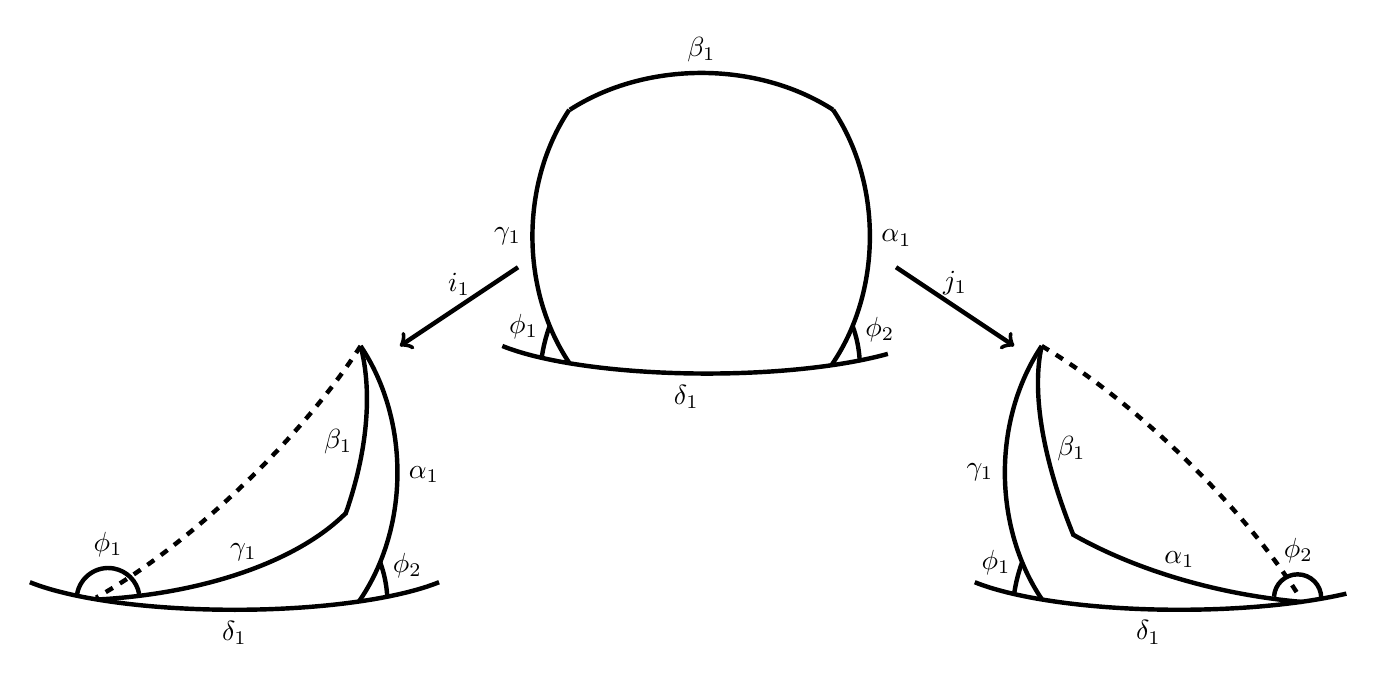
\begin{tikzpicture}
        \draw[ultra thick] (6.8, 3) arc[start angle=210, end angle = 320, x radius = 3cm, y radius = 0.7cm]  node[below, midway] {$\delta_1$};
        \draw[ultra thick] (7.65, 6) arc [start angle=140, end angle=220,x radius = 2cm, y radius = 2.5cm] node[left, midway] {$\gamma_1$};
        \draw[ultra thick] (11, 6) arc [start angle=40, end angle=-41,x radius = 2cm, y radius = 2.5cm] node[right, midway] {$\alpha_1$};
        \draw[ultra thick] (11,6) arc [start angle=50, end angle=130,x radius =2.6cm, y radius = 2cm] node[above, midway] {$\beta_1$};
        \draw[ultra thick] (7.4, 3.25) arc[start angle = 160, end angle = 172,radius=2cm] node[left, pos = 0] {$\phi_1$};
        \draw[ultra thick] (11.25, 3.25) arc[start angle = 20, end angle = 3,radius=1.5cm] node[right, pos = 0.1] {$\phi_2$};

        \draw[->, ultra thick] (7, 4) -- (5.5,3) node[above, midway] {$i_1$};
        
        \draw[ultra thick] (0.8, 0) arc[start angle=210, end angle = 330, x radius = 3cm, y radius = 0.7cm]  node[below, midway] {$\delta_1$};
        \draw[ultra thick] (1.65, -0.22) arc [start angle = -84, end angle = -26.5, x radius = 4cm, y radius = 2cm] node[above, midway] {$\gamma_1$};
        \draw[ultra thick] (5, 3) arc [start angle=40, end angle=-41,x radius = 2cm, y radius = 2.5cm] node[right, midway] {$\alpha_1$};
        \draw[ultra thick, rotate around = {-30:(5,3)}] (5,3) arc [start angle=60, end angle = 18,x radius =2cm, y radius = 3.5cm] node[left, pos=0.6] {$\beta_1$};
        \draw[ultra thick] (1.4, -0.15) arc[start angle = 170, end angle = 10,radius=0.4cm] node[above, pos = 0.5] {$\phi_1$};
        \draw[ultra thick] (5.25, 0.25) arc[start angle = 20, end angle = 3,radius=1.5cm] node[right, pos = 0.1] {$\phi_2$};
         \draw[ultra thick, dashed, rotate around = {-46:(5,3)}] (5, 3) arc[start angle=40, end angle=-43,x radius = 1cm, y radius = 3.5cm];

         \draw[->, ultra thick] (11.8, 4) -- (13.3,3) node[above, midway] {$j_1$};

        %\node [green] at (17.2, 1.8) {\textbullet};
        
        \draw[ultra thick] (12.8, 0) arc[start angle=210, end angle = 315, x radius = 3cm, y radius = 0.7cm]  node[below, midway] {$\delta_1$};
        \draw[ultra thick] (13.65, 3) arc [start angle=140, end angle=220,x radius = 2cm, y radius = 2.5cm] node[left, midway] {$\gamma_1$};
        \draw[ultra thick, rotate around = {80:(16.95, -0.25)}] (16.95, -0.25) arc [start angle=190, end angle=144.5,x radius = 2cm, y radius = 4cm] node[above, midway] {$\alpha_1$};
        \draw[ultra thick, rotate around = {-55:(13.65, 3)}] (13.65, 3) arc [start angle=200, end angle=240,x radius =5cm, y radius = 2cm] node[right, pos = 0.6] {$\beta_1$};
        \draw[ultra thick] (13.4, 0.25) arc[start angle = 160, end angle = 172,radius=2cm] node[left, pos = 0] {$\phi_1$};
        \draw[ultra thick] (17.2, -0.2) arc[start angle = 0, end angle = 177, radius=0.3cm] node[above, pos = 0.5] {$\phi_2$};
         \draw[ultra thick, dashed, rotate around = {46:(13.65, 3)}] (13.65, 3) arc[start angle=40, end angle=-42, x radius = 1cm, y radius = 3.5cm];
    \end{tikzpicture}
}
    \caption{Action of involutions on a spherical quadrilateral}
    \label{fig6}
\end{figure}
$$
\begin{matrix}
i_1:(x_2, x_1) \to (x_2, x'_1), & j_1:(x_2, x_1) \to (x'_2, x_1)
\end{matrix}
$$
act by folding the quadrilateral along one of its diagonals, see \cref{fig6}.
Then the involutive coupling of quadrilaterals implies compatibility of the involutions $j_1$ and $j_2$ (or the condition \cref{eq10} on the involution factors) for the coupling $(Q_1, Q_2)$. In geometrical terms it can be interpreted as conditions on the angles $\xi_1, \xi_2, \xi_1', \xi_2'$, which are expressed in the following result.
\begin{figure}[ht!]
    \centering
    \scalebox{0.8}{
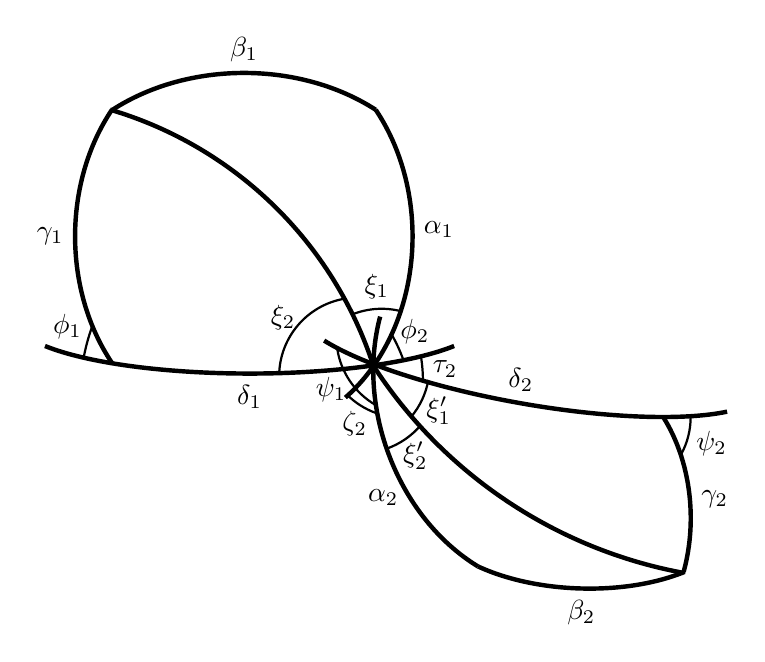
\begin{tikzpicture}
     \draw[ultra thick] (0.5, 2) arc[start angle=210, end angle = 330, x radius = 3cm, y radius = 0.7cm]  node[below, midway] {$\delta_1$};
        \draw[ultra thick] (1.35, 5) arc [start angle=140, end angle=220,x radius = 2cm, y radius = 2.5cm] node[left, midway] {$\gamma_1$};
        \draw[ultra thick] (4.7, 5) arc [start angle=40, end angle=-55,x radius = 2cm, y radius = 2.5cm] node[right, pos = 0.4] {$\alpha_1$};
        \draw[ultra thick] (4.7,5) arc [start angle=50, end angle=130,x radius =2.6cm, y radius = 2cm] node[above, midway] {$\beta_1$};
        \draw[thick] (1.1, 2.25) arc[start angle = 160, end angle = 170,radius=2.5cm] node[left, pos = 0] {$\phi_1$};
        \draw[thick] (4.9, 2.15) arc[start angle = 30, end angle = 20,radius=2cm] node[right, pos = -0.1] {$\phi_2$};
        
%        \node [red] at (11.7, 1.75) {\textbullet};
%        \node [red] at (15.35, 1.1) {\textbullet};
%        \node [green] at (13,-0.8) {\textbullet};
 %       \node [green] at (11.8, 1) {\textbullet};
        
        
        \draw[ultra thick, rotate around={-10:(4.7,1.75)}] (4, 1.95) arc [start angle=210, end angle = 330, x radius = 3cm, y radius = 0.7cm] node[above, midway] {$\delta_2$};
        \draw[ultra thick, rotate around = {19:(6,-0.8)}] (6,-0.8) arc [start angle=-134, end angle=-220,x radius = 2cm, y radius = 2.5cm] node[left, pos = 0.35] {$\alpha_2$};
        \draw[ultra thick, rotate around = {0:(8.35,1.1)}] (8.35,1.1) arc [start angle=40, end angle=-20,x radius = 1.5cm, y radius = 2cm] node[right, pos = 0.55] {$\gamma_2$};
        \draw[ultra thick, rotate around = {-2:(6,-0.8)}] (6,-0.8) arc [start angle=230, end angle=312,x radius = 2cm, y radius = 1cm] node[below, midway] {$\beta_2$};
        \draw[thick] (5.3, 1.55) arc[start angle = 0, end angle = 9,radius=2cm] node[right, pos = 0.5] {$\tau_2$};
        \draw[thick] (4.7, 1.25) arc[start angle = -120, end angle = -171,radius=1cm] node[left, pos = 0.35] {$\psi_1$};
        \draw[thick] (8.7, 1.1) arc[start angle = 0, end angle = -28, radius=1cm] node[right, pos = 0.7] {$\psi_2$};
        \draw[thick] (4.7, 1.15) arc[start angle = -110, end angle = -135, radius=1cm] node[below, pos = 0.7] {$\zeta_2$};
        \draw[ultra thick, rotate around = {18:(4.67, 1.75)}] (4.67, 1.75) arc[start angle = 0, end angle = 55.6, radius = 5cm];
        \draw[ultra thick, rotate around = {-147:(4.67, 1.75)}] (4.67, 1.75) arc[start angle = 0, end angle = 46.5, radius = 6cm];
        \draw[thick] (4.4, 2.4) arc[start angle = 112, end angle = 75, radius = 1cm] node[above, pos = 0.5] {$\xi_1$};
        \draw[thick] (4.3, 2.6) arc[start angle = 100, end angle = 179, radius = 1cm] node[left, pos = 0.4] {$\xi_2$};
        \draw[thick] (5.15, 1.1) arc[start angle = -40, end angle = -10, radius = 1cm]  node[right, pos = 0.2] {$\xi'_1$};
        \draw[thick] (4.85, 0.7) arc[start angle = -70, end angle = -40, radius = 1cm]  node[below, pos = 0.8] {$\xi'_2$};
    \end{tikzpicture}
}
    \caption{Illustration of Lemma~\ref{lem-final}}
    \label{fig7}
\end{figure}

\begin{lemma} \label{lem-final}
Let the spherical elliptic orthodiagonal quadrilaterals $Q_1$ and $Q_2$ form an involutive coupling as in \cref{fig7}. Then
$$
\begin{matrix}
\xi_1 = \xi_1' + \tau_2 + \zeta_2, &
\xi_2 = \xi_2'
\end{matrix},
$$
during flexions.
\end{lemma}
\begin{proof}
The condition \cref{eq10} means compatibility of the involutions $j_1$ and $j_2$. This is geometrically equivalent to the following condition on the angles 
\begin{equation*}
\xi_1 - \xi_2 = \xi_1' - \xi_2' + \tau_2 + \zeta_2.
\end{equation*}
Also, from the construction of the linkage $(Q_1, Q_2)$ we have that $\xi_1 + \xi_2 = \xi_1' + \xi_2' + \tau_2 + \zeta_2$.
\end{proof}

\section{Conclusion}

In this paper we have shown how to generalize Izmestiev's method towards SQ Kokotsakis polyhedra. By doing this, we constructed the class of SQ $3 \times 3$ complexes of orthodiagonal involutive type. This remarkable class plays an important role in Izmestiev's classification. We exploited his method for the study of the Bricard polynomial system. Izmestiev's classification is based on the commutative diagram of branched covers of projection maps between configuration spaces of one, two and all spherical quadrilaterals. The OI type is based on the subdiagram where projections from $Z_{12}, Z_{34}$ to $Z_2, Z_4$ are two-fold. The Bricard system in the skew case differs from the planar case in some terms, but not in total degree, which implies that the diagram remains the same. As it was shown in previous sections, we were able to derive conditions for the  skew case by studying the same subdiagram, though, not explicitly mentioning it.

Therefore, all SQ Kokotsakis polyhedra may be classified similiar to Izmestiev's classification, potentially adding new subclasses to some families. However, as algebraic computations in the skew case become more complicated, we leave a complete classification for future work.

\section{Acknowledgements}

The authors are grateful to Caigui Jiang for the graphical vizualization of flexible polyhedra. This work has been supported by KAUST baseline funding. Alisher Aikyn acknowledges KAUST support and the hospitality during his research stay at KAUST.

\bibliographystyle{unsrt}
\bibliography{main}

\newpage
\appendix
\section{Deltoids and antideltoids}
\label{sec:appendix}


\subsection{OI type with two (anti)deltoids}
\begin{enumerate}
    \item Planar angles $(\alpha_i , \beta_i, \gamma_i, \delta_i)$, where $i = 1, 4$, satisfy the conditions:
    $$
    \begin{matrix}
    \cos(\alpha_i) \cos(\gamma_i) = \cos(\beta_i) \cos(\delta_i) & \alpha_i \pm \beta_i \pm \gamma_i \pm \delta_i \neq 0 \text{ mod } 2\pi
    \end{matrix}
    $$
    and planar angles $(\alpha_i, \beta_i, \gamma_i, \delta_i)$, where $i =2, 3$, both satisfy one of the conditions:
    \begin{equation*}
        \begin{matrix}
            \alpha_i = \beta_i\text{, } & \gamma_i = \delta_i & \text{or} & \alpha_i = \pi - \beta_i\text{, } & \gamma_i = \pi - \delta_i
        \end{matrix}    
    \end{equation*}
    \item The couplings of adjacent quadrilaterals are compatible, see~\cref{def3.6};
    \item The set of parameters $(\nu_1, \xi_2, \xi_3, \nu_4, t_1, t_2, F_3, t_4)$ satisfies the following system, where in $\pm$ the first sign is chosen if $Q_2, Q_3$ are deltoids or the second otherwise,
    \begin{equation*}\label{eq24}
        \begin{gathered}
            p_{12} = -2 \xi_3 \nu_4 t_1 t_2 t_4 + 2 \xi_2 \nu_4 t_1 + 8 \xi_3 t_2 + 8 \xi_2 t_4 \pm F_3(4 \nu_4 t_1 t_2 + \xi_2 \xi_3 \nu_4 t_1 t_4 + 16 t_2 t_4 - 4 \xi_2 \xi_3),\\
            p_{13} = \xi_3(-\nu_1 \xi_2 \nu_4 t_1 t_2 t_4 + 16  \xi_2 t_1 + 4 \nu_1 \xi_2 t_2 + 4 \xi_2 \nu_4 t_4 \pm F_3(32 t_1 t_2 + 2 \nu_1 \nu_4 t_1 t_4 + 8 \nu_4 t_2 t_4 - 8 \nu_1)),\\
            p_{14} =  2(16 \xi_2 - \nu_1 \xi_3 \nu_4) t_1 t_4 + 8(\nu_1 \xi_3 - \xi_2 \nu_4) \pm F_3((64 - \nu_1 \xi_2 \xi_3 \nu_4) t_1 t_2 t_4 + 4( \nu_1 \xi_2 \xi_3 - 4 \nu_4) t_2),\\
            p_{23} = (\nu_1 \xi_2 \nu_4 - 16 \xi_3) t_1 t_2 + 4 (\nu_1 \xi_2 - \xi_3 \nu_4) t_2 t_4 \pm F_3(2 (4 \xi_2 \xi_3 - \nu_1 \nu_4) t_1 + 2 (\xi_2 \xi_3 \nu_4 - 4 \nu_1) t_4),\\
            p_{24} = -64 t_1 t_2 t_4  + 4 \nu_1 \nu_4 t_1 + 16 \nu_4 t_2 + 16 \nu_1 t_4 \pm F_3(2 \nu_1 \xi_2 \nu_4 t_1 t_2 + 32 \xi_2 t_1 t_4 + 8 \nu_1 \xi_2 t_2 t_4 - 8 \xi_2 \nu_4),\\
            p_{34} = \nu_1 (-8 \xi_2 t_1 t_2 t_4 + 8\xi_3 t_1 + 2 \xi_2 \nu_4 t_2 + 2 \xi_3 \nu_4 t_4 + F_3(4 \xi_2 \xi_3 t_1 t_2 + 16 t_1 t_4 + \xi_2 \xi_3 \nu_4 t_2 t_4 - 4 \nu_4)).
        \end{gathered}    
    \end{equation*}
\end{enumerate}
\subsection{OI type with deltoid and antideltoid}\label{secA2}
This subclass has no counterpart in the planar case.  
\begin{enumerate}
     \item Planar angles $(\alpha_i , \beta_i, \gamma_i, \delta_i)$, $i = 1, 4$, satisfy the conditions:
    $$
    \begin{matrix}
    \cos(\alpha_i) \cos(\gamma_i) = \cos(\beta_i) \cos(\delta_i) & \alpha_i \pm \beta_i \pm \gamma_i \pm \delta_i \neq 0 \text{ mod } 2\pi
    \end{matrix}
    $$
    and planar angles $(\alpha_i, \beta_i, \gamma_i, \delta_i)$, where $i = 2, 3$, satisfy the conditions:
    \begin{equation*}
        \begin{matrix}
            \alpha_2 = \beta_2\text{, } & \gamma_2 = \delta_2\text{, } & \alpha_3 = \pi - \beta_3\text{, } & \gamma_3 = \pi - \delta_3
        \end{matrix}
    \end{equation*}
    \item The couplings of adjacent quadrilaterals are compatible, see~\cref{def3.6};
    \item\label{eq25} The set of parameters $(\nu_1, \xi_2, \xi_3, \nu_4, t_1, t_2, F_3, t_4)$ satisfies the system
    \begin{equation*}
        \begin{gathered}
            p_{12} = -2 \xi_3 \nu_4 t_1 t_2 F_3 t_4 + 4 \nu_4 t_1 t_2 - 2 \xi_2 \nu_4 t_1 F_3 - \xi_2 \xi_3 \nu_4 t_1 t_4 + 8 \xi_3 t_2 F_3 + 16 t_2 t_4 - 8 \xi_2 F_3 t_4 + 4 \xi_2 \xi_3,\\
            p_{13} = 32 t_1 t_2 F_3 t_4 + \nu_1 \xi_2 \nu_4 t_1 t_2 - 2 \nu_1 \nu_4 t_1 F_3 + 16 \xi_2 t_1 t_4 - 8 \nu_4 t_2 F_3 + 4 \nu_1 \xi_2 t_2 t_4 - 8 \nu_1 F_3 t_4 - 4 \xi_2 \nu_4,\\
            p_{14} = \nu_1 \xi_2 \nu_4 t_1 t_2 F_3 + 16 \xi_3 t_1 t_2 F_3 + 4 \xi_3 \nu_4 t_2 F_3 t_4 + 4 \nu_1 \xi_2 t_2 F_3 t_4 + 8 \xi_2 \xi_3 t_1 + 2 \nu_1 \nu_4 t_1 + 2 \xi_2 \xi_3 \nu_4 t_4 +8 \nu_1 t_4,\\
            p_{23} = (\nu_1 \xi_2 \xi_3 \nu_4 + 64) t_1 t_2 t_4 - 2(16 \xi_2 + \nu_1 \xi_3 \nu_4) t_1 F_3 t_4 - 4(4 \nu_4 + \nu_1 \xi_2 \xi_3)t_2 + 8 (\xi_2 \nu_4 + \nu_1 \xi_3) F_3,\\
            p_{24} = \xi_3 (\nu_1 \xi_2 \nu_4 t_1 t_2 F_3 t_4 + 32 t_1 t_2 - 16 \xi_2 t_1 F_3 + 2 \nu_1 \nu_4 t_1 t_4 - 4 \nu_1 \xi_2 t_2 F_3 +  8 \nu_4 t_2 t_4 - 4 \xi_2 \nu_4 F_3 t_4 - 8 \nu_1),\\
            p_{34} = \nu_1 (8 \xi_2 t_1 t_2 F_3 t_4 - 4 \xi_2 \xi_3 t_1 t_2 + 8 \xi_3 t_1 F_3 + 16 t_1 t_4 - 2 \xi_2 \nu_4 t_2 F_3 - \xi_2 \xi_3 \nu_4 t_2 t_4 + 2 \xi_3 \nu_4 F_3 t_4 - 4 \nu_4).
        \end{gathered}
    \end{equation*}    
\end{enumerate}
\textbf{Example.}
Here we present the dihedral and planar angles for a flexible Kokotsakis polyhedron of OI type with deltoid and antideltoid. The example is constructed under the assumption that $t_1 t_2 t_4 \neq 0$, $F_3 \neq 0$ with the following angles
\begin{figure}[ht!]
        \centering
        \includegraphics[width=15cm]{deltoid-antideltoid.png}
        \caption{Some positions of a deltoid-antideltoid polyhedron, exhibiting self-intersections.}
\end{figure}
\begin{equation*}
    \begin{matrix}
        \delta_1 = \frac{\pi}{3}, & \delta_2 = \arccos\frac{\sqrt{3}}{4}, & \delta_3 = \frac{2\pi}{3}, & \delta_4 = \arccos\frac{\sqrt{3}}{4},\\
    \end{matrix}
\end{equation*}
\begin{equation*}
    \begin{matrix}
        \tau_1 = \arccos\frac{3}{\sqrt{13}},& \tau_2 = \arccos\frac{3}{\sqrt{13}},& \tau_3 = \arccos\frac{1}{13},& \tau_4 = \arccos\frac{1}{13},
    \end{matrix}
\end{equation*}
\begin{equation*}
    \begin{matrix}
        t_1 = 10,& t_2 = \frac{-3597+2600\sqrt{3}}{5(39 + 12218\sqrt{3})}, & F_3 = \frac{1}{10}, & t_4 = \frac{-3597+2600\sqrt{3}}{-5(39 + 12218\sqrt{3})},
    \end{matrix}
\end{equation*}
\begin{equation*}
    \begin{matrix}
        \zeta_1 = \arctan t_1 - \tau_1,& \zeta_2 = \arctan t_2 - \tau_2,& \zeta_3 = 2\arctan F_3 - \tau_3,& \zeta_4 = \arctan t_4 - \tau_4,\\
    \end{matrix}
\end{equation*}
\begin{equation*}
    \alpha_1 = \alpha_2 = \alpha_3 = \alpha_4 = \frac{\pi}{2}, \quad \gamma_1 = \gamma_2 = \gamma_3 = \gamma_4 = \frac{\pi}{2}, \quad \beta_1 = \beta_2 = \beta_3 = \beta_4 = \frac{\pi}{2}.
\end{equation*}


\end{document}
